\documentclass[11pt, a4paper]{article}

% Packages
\usepackage[hmargin=2.5cm, vmargin=3cm]{geometry} % hmargin=73.5pt, vmargin=85pt

\usepackage[T1]{fontenc}    % Encodage des accents
\usepackage[utf8]{inputenc} % Lui aussi
\usepackage[square,sort,colon,authoryear]{natbib}         % Pour la bibliographie
%\setcitestyle{square}
% \usepackage[frenchb]{babel} % Pour la traduction française
\usepackage[english, main=frenchb]{babel}
%\frenchbsetup{IndentFirst=true}
%\frenchbsetup{StandardLayout=true}  % in case French is the main language, not to modify layout of lists
\frenchbsetup{GlobalLayoutFrench=false}  %  in case French is the main language, to apply modification to lists only in parts of the document using French


\usepackage{enumitem}       % Pour modifier l'espace avant/après les listes

\usepackage{url}            % Pour citer les adresses web
\usepackage{hyperref}       % Pour activer les liens cliquables

% Package pour avoir la section Annexes
\usepackage{appendix}
%\renewcommand{\appendixtocname}{Annexes}  % On renomme dans la table des matières
%\renewcommand{\appendixpagename}{Annexes} % On renomme dans le document
%\usepackage{numprint}  % Histoire que les chiffres soient bien
\usepackage{eurosym}  % Permet l'utilisation du signe €
% Exemple : \EUR{\num{299792458.38}}

\usepackage[maxlevel=3]{csquotes}  % Propose des commandes pour les citations. L'option maxlevel permet de déterminer le nombre de niveaux d'imbrication maximal.
% Exemple :  \enquote{Lorsque yyy déclare \enquote{zzz} il ne déclare rien du tout}. Les citations en bloc sont également possible : \begin{quote} citation \end{quote}. Pour les citations plus longues, on préfèrera \begin{quotation} citation longue \end{quotation}. 
\usepackage{setspace}  % Permet de modifier l'espacement entre les lignes.
\usepackage{siunitx}  % Pareil que numprint, mais pour un cadre mathématiques, donc permet de faire plus de chose : http://ctan.mines-albi.fr/macros/latex/contrib/siunitx/siunitx.pdf

\sisetup{locale = UK} % Permet de selectionner le type de convention (UK, US, FR)
% Exemples :
%\num{299792458} :  Il y a des espaces.
%\num{299792,458} : On obtient une virgule comme séparateur décimal.
%\num{.34} : Même en utilisant le point, on obtient une virgule et un zéro est placé.
%\num{299792,458 +- 0.09} : on peut obtenir le signe « plus ou moins » avec +-.
%\num{3e8} : « e » permet d’obtenir la puissance de 10, avec le signe x (3 x 10^8)

%\usepackage[
%    left = \flqq{},% 
%    right = \frqq{},% 
%    leftsub = \flq{},% 
%    rightsub = \frq{} %
%]{dirtytalk}
\usepackage{dirtytalk}
\usepackage{amsthm}
%\theoremstyle{theorem}
%\newtheorem{theorem}{Théorème}[chapter]

%\theoremstyle{theorem}
%\newtheorem{prop}{Propriété}[chapter]

%\theoremstyle{theorem}
%\newtheorem{proposition}{Proposition}[chapter]

%\theoremstyle{theorem}
%\newtheorem{corollaire}{Corollaire}[chapter]

%\theoremstyle{lemma}
%\newtheorem{lemma}{Lemme}[chapter]

%\theoremstyle{definition}
%\newtheorem{definition}{Définition}[chapter]

%\theoremstyle{exemple}
%\newtheorem{exemple}{Exemple}[chapter]

%\theoremstyle{remarque}
%\newtheorem{remarque}{Remarque}[chapter]

\usepackage{amsmath}        % La base pour les maths
\usepackage{mathrsfs}       % Quelques symboles supplémentaires
\usepackage{amssymb}        % encore des symboles.
\usepackage{amsfonts}       % Des fontes, eg pour \mathbb.
\usepackage{mathtools}      % Permet d'utiliser des symboles d'égalités spéciaux
\usepackage{centernot}
\usepackage{dsfont}         % Pour avoir les notations nécessaires aux ensembles (nécessite mathbb)
\usepackage{stmaryrd}       % Permet de faire des intervalles avec des doubles barres (intervalles d'entiers)
\usepackage{esvect}         % Donne plein de possibilité pour les flèches des vecteurs
\usepackage{systeme}        % Permet de créer facilement des systèmes (en mode mathématique ou en texte)
\usepackage{bm}
\usepackage{stmaryrd}
\SetSymbolFont{stmry}{bold}{U}{stmry}{m}{n}

\usepackage{xspace}         % Utile lors de la création d'abréviations
\usepackage{verbatim}       % Permet d'insérer du code LaTeX sans qu'il soit compilé

% Packages pour la création de nouvelles commandes
\usepackage{xifthen}
\usepackage{xargs}
% Packages pour images et graphiques
\usepackage{graphicx}   % inclusion des graphiques
\usepackage{wrapfig}    % Dessins dans le texte.
\usepackage{caption}    % Permet de personnaliser les styles des légendes.
\usepackage{subcaption} % Permet d’insérer au sein d’une figure des sous-figures, chacune d’entre elles disposant d’une légende, en plus de la légende principale.
\newcommand{\source}[1]{\vspace{-8pt} \caption*{ Source: {#1}} }

\makeatletter
\newcommand*{\centerfloat}{%
  \parindent \z@
  \leftskip \z@ \@plus 1fil \@minus \textwidth
  \rightskip\leftskip
  \parfillskip \z@skip}
\makeatother

\usepackage{color}
\usepackage{array}
\usepackage[table]{xcolor}
\newcommand{\HRule}{\rule{\linewidth}{0.5mm}}

% Un package pour les dessins (utilisé pour l'environnement {code})
\usepackage{tikz}     
\usepackage[framemethod=TikZ]{mdframed}
\usepackage{pgfplots}
\pgfplotsset{compat=1.14}
%\pgfplotsset{compat=1.17}

% documentation of the package
% https://distrib-coffee.ipsl.jussieu.fr/pub/mirrors/ctan/macros/latex/contrib/algorithm2e/doc/algorithm2e.pdf
\usepackage[ruled,vlined]{algorithm2e}


% Permet de rentrer du code dans le document
% Permet de rentrer du code dans le document

\usepackage{listings}
\usepackage{listingsutf8}
\usepackage{color}
\definecolor{truegreen}{rgb}{0.2,0.7,0.2}
\definecolor{trueorange}{rgb}{1,0.6,0.1}
\definecolor{truepink}{rgb}{1,0,0.6}
\definecolor{codegreen}{rgb}{0,0.6,0}
\definecolor{codegray}{rgb}{0.5,0.5,0.5}
\definecolor{codepurple}{rgb}{0.58,0,0.82}
\definecolor{backcolour}{rgb}{0.95,0.95,0.92}
\definecolor{codegreen}{rgb}{0,0.6,0}
\definecolor{codegray}{rgb}{0.5,0.5,0.5}
\definecolor{codepurple}{rgb}{0.58,0,0.82}
\definecolor{backcolour}{rgb}{0.95,0.95,0.92}

\newcommand{\txcr}[1]{\textcolor{red}{#1}}
\newcommand{\txcg}[1]{\textcolor{blue}{#1}}
\newcommand{\txog}[1]{\textcolor{black}{#1}}
 
\lstdefinestyle{mystyle}{
    backgroundcolor=\color{backcolour},   
    commentstyle=\color{codegreen},
    keywordstyle=\color{magenta},
    numberstyle=\tiny\color{codegray},
    stringstyle=\color{codepurple},
    basicstyle=\footnotesize,
    breakatwhitespace=false,         
    breaklines=true,                 
    captionpos=b,                    
    keepspaces=true,                 
    numbers=left,                    
    numbersep=5pt,                  
    showspaces=false,                
    showstringspaces=false,
    showtabs=false,                  
    tabsize=2
}
\lstset{
    style = mystyle,
    language = Python,
    extendedchars,
    showstringspaces=false,
    literate=%
         {à}{{\`a}}1
         {é}{{\'e}}1
         {è}{{\`e}}1
         {ê}{{\^e}}1
         {ô}{{\^o}}1
         {ù}{{\`u}}1
         {î}{{\^i}}1
}

% New commands
%%%%%%%%%%%%%%%%%%%%%%%%%%%%%%%%%%%%%%%%%%%%%%%%
% Ce fichier contient des nouvelles commandes 
% pour faciliter l'écriture des mathématiques
%%%%%%%%%%%%%%%%%%%%%%%%%%%%%%%%%%%%%%%%%%%%%%%%

% Ensembles
\let\ensembleNombre\mathbb
\newcommand*\N{\ensuremath{\ensembleNombre{N}}}       % Ensemble des entiers naturels N
\newcommand*\Z{\ensuremath{\ensembleNombre{Z}}}       % Ensemble des entiers relatifs Z
\newcommand*\Q{\ensuremath{\ensembleNombre{Q}}}       % Ensemble des rationnels Q
\newcommand*\R{\ensuremath{\ensembleNombre{R}}}       % Ensemble des réels R
\newcommand*\Complex{\ensuremath{\ensembleNombre{C}}} % Ensemble des complexes C

% Encadrement
\newcommand{\angles}[1]{\left\langle #1 \right\rangle} % ⟨⟩
\newcommand{\braces}[1]{\left\lbrace #1 \right\rbrace} % {}
\newcommand{\bracks}[1]{\left\lbrack #1 \right\rbrack} % []
\newcommand{\pars}[1]{\left( #1 \right)}               % ()
\newcommand{\norme}[1]{\left\Vert #1\right\Vert}       % Norme
\newcommand{\ent}[1]{\left\lfloor #1\right\rfloor}     % Partie entière inférieure
\newcommand{\entsup}[1]{\left\lceil #1\right\rceil}    % Partie entière supérieure
\newcommand{\abs}[1]{\left\vert #1\right\vert}         % Valeur absolue

% Dérivées
\newcommand{\deriv}[3][]{\frac{\mathrm{d}^{#1}#2}{\mathrm{d} {#3}^{#1}}}    % Dérivée non partielle  
\newcommand{\partiald}[3][]{\frac{\partial^{#1}#2}{\partial {#3}^{#1}}} % Dérivée partielle   

% Intervalles
\newcommand*\intervalle[4]{\left#1 #2 \, ; #3 \right#4}                       % Définit la notion d'intervalle
\newcommand*\intervalleOO[2]{\intervalle{(}{#1}{#2}{)}}                       % ]a ; b[
\newcommand*\intervalleFF[2]{\intervalle{[}{#1}{#2}{]}}                       % [a ; b]
\newcommand*\intervalleOF[2]{\intervalle{(}{#1}{#2}{]}}                       % ]a ; b]
\newcommand*\intervalleFO[2]{\intervalle{[}{#1}{#2}{)}}                       % [a ; b[
\newcommand*\intervalleEntier[2]{\intervalle{\llbracket}{#1}{#2}{\rrbracket}} % Ensemble d'entiers

% Ensemble "tel que"
\newcommand*\enstq[2]{\braces{#1,\; #2}}                                      

% Probabilité, espérance, variance, covariance et corrélation
\newcommandx{\proba}[3][1, 3=0]{
\ifthenelse{\isempty{#2}}{\mathbb{P}_{#1}}{%
\ifthenelse{\equal{#3}{0}}{\mathbb{P}_{#1}\pars{#2}}{\mathbb{P}_{#1}\pars{#2 \middle| #3}}}%
}
\newcommandx{\esp}[3][1, 3=0]{
\ifthenelse{\isempty{#2}}{\mathbb{E}_{#1}}{%
\ifthenelse{\equal{#3}{0}}{\mathbb{E}_{#1}\bracks{#2}}{\mathbb{E}_{#1}\bracks{#2 \middle| #3}}}%
}
\newcommandx{\var}[3][1, 3=0]{
\ifthenelse{\isempty{#2}}{\operatorname{Var}_{#1}}{%
\ifthenelse{\equal{#3}{0}}{\operatorname{Var}_{#1}\pars{#2}}{\operatorname{Var}_{#1}\pars{#2 \middle| #3}}}%
}
\newcommandx{\cov}[4][1, 4=0]{
\ifthenelse{\isempty{#2} \AND \isempty{#3}}{\operatorname{Cov}_{#1}}{%
\ifthenelse{\equal{#4}{0}}{\operatorname{Cov}_{#1}\pars{#2, #3}}{\operatorname{Cov}_{#1}\pars{#2, #3 \middle| #4}}}%
}
\newcommandx{\corr}[3][1]{\ifthenelse{\isempty{#2} \AND \isempty{#3}}{\operatorname{Corr}_{#1}}{\operatorname{Corr}_{#1}\pars{#2, #3}}}

% Lois usuelles de probabilités
\newcommand{\Ber}[1]{\mathcal{B}ernoulli\pars{#1}}
\newcommand{\Binom}[2]{\mathcal{B}\pars{#1, #2}}
\newcommand{\Poisson}[1]{\mathcal{P}\pars{#1}}
\newcommand{\Geo}[1]{\mathcal{G}eo\pars{#1}}
\newcommand{\Unif}[1]{\mathcal{U}nif_{#1}}
\newcommand{\Exp}[1]{\mathcal{E}xp\pars{#1}}
\newcommandx{\Norm}[3][1]{\mathcal{N}_{#1}\pars{#2, #3}}
\newcommand{\Gam}[2]{\Gamma\pars{#1, #2}}
\newcommand{\InvGam}[2]{\text{Inv-}\Gamma\pars{#1, #2}}
\newcommand{\Betaloi}[2]{\beta\pars{#1, #2}}
\newcommand{\Pareto}[2]{\mathcal{P}areto\pars{#1, #2}}
\newcommand{\Laplace}[1]{\mathcal{L}\pars{#1}}
\newcommand{\Cauchy}[1]{\mathcal{C}\pars{#1}}

% Égalités
\newcommandx{\egalloi}{\overset{\mathrm{\mathcal{L}oi}}{=}}
\newcommandx{\egalprob}{\overset{\mathbb{P}}{=}}
\newcommandx{\egaltxt}[1]{\overset{\mathrm{#1}}{=}}
\newcommandx{\simiid}{\overset{\mathrm{iid}}{\sim}}

% Indicatrice
\newcommand{\1}[1][]{\mathds{1}_{\braces{#1}}}

% max, min, argmax et argmin avec subscript
\newcommandx{\maxx}[1]{\underset{#1}{\max}}
\newcommandx{\minn}[1]{\underset{#1}{\min}}
\newcommandx{\argmax}[1][1]{\underset{#1}{\arg\max}}
\newcommandx{\argmin}[1][1]{\underset{#1}{\arg\min}}

% matrice 3*3 diagonale avec la diagonale donnée sur les 3 arguments
\newcommand{\mattroisdiag}[3]{\left( \begin{array}{ccc} #1 &  0 &  0 \\ 0  & #2 &  0 \\ 0  &  0 & #3\end{array} \right)}

% Intégration
\newcommand{\dint}{\mathrm{d}}
\newcommandx{\integ}[4][2]{\int_{#1}^{#2} #3 \, \mathrm{d} #4} 

% moyenne simple et quadratique d'une grandeur scalaire
\newcommand{\moy}[1]{\overline{#1}}
\newcommand{\moyy}[1]{\overline{#1^2}}

% Vecteurs
\let\vecteur\overrightarrow % Permet de modifier la taille de la flèche d'un vecteur quand ce dernier est composé de plusieurs lettres par exemple.
\newcommand*\coord[2]
{
   \vecteur{#1} \,
   \begin{pmatrix}
      #2
   \end{pmatrix}
} % Permet de déclarer les coordonnées d'un vecteur, exemple : \[\coord{AB}{12\\21} \coord{BC}{21\\12\\32}\]

% Surface et volume
\newcommandx{\surf}[2][2=m]{\numprint{#1}\,#2\textsuperscript{2}}
\newcommandx{\vol}[2][2=m]{\numprint{#1}\,#2\textsuperscript{3}}

% Fonction
%\newcommand*\fonction[5]{
%#1 \colon \left\{\begin{alignedat}{2}  &#2 &\: &\to      #3\\
%                                &#4 &   &\mapsto  #5
%\end{alignedat} \right. \kern-\nulldelimiterspace} % Permet de déclarer facilement une fonction, exemple : $\fonction{f}{E}{F}{x}{f(x)}$

\newcommand*\fonction[5]{\begin{align*}#1 \colon #2 & \to #3\\#4 & \mapsto #5\end{align*}} 
% Permet de déclarer facilement une fonction, exemple : $\fonction{f}{E}{F}{x}{f(x)}$

\newcommand{\twopartdef}[4]
{
	\left\{
		\begin{array}{ll}
			#1 & \mbox{si } #2 \\
			#3 & \mbox{si } #4
		\end{array}
	\right.
}

\newcommand{\threepartdef}[6]
{
	\left\{
		\begin{array}{lll}
			#1 & \mbox{si } #2 \\
			#3 & \mbox{si } #4 \\
			#5 & \mbox{si } #6
		\end{array}
	\right.
}

% Autres commandes utiles
\newcommand{\compos}{\circ}                 % operateur de composition de fonctions
\DeclareMathOperator{\card}{card}           % On déclare l’opérateur \card qui correspond à « card ».
\newcommand*\PI{\ensuremath{\pi}}           % Permet d'afficher pi que l'on soit en mode math ou non.
\newcommand{\ds}[1]{\displaystyle{#1}}      % Force LaTeX à gérer les indices et les exposants comme si il était en mode mathématique isolé
% fonction exponentielle
\newcommand{\e}[1]{\exp{\pars{#1}}}

\newcommand{\kronecker}[0]{\mathrm{\delta}} % symbole de Kronecker
\newcommand{\heaviside}[0]{\mathrm{H}}      % fonctions d'Heaviside
\newcommand{\dirac}[0]{\mathrm{\delta}}     % Distribution de Dirac

\newcommand*{\TakeFourierOrnament}[1]{{%
\fontencoding{U}\fontfamily{futs}\selectfont\char#1}}
\newcommand*{\danger}{\TakeFourierOrnament{66}}
%%%%%%%%%%%%%%%%%%%%%%%%%%%%%%%%%%%%%%%%%%%%%%%%
% Ce fichier contient des commandes pour respecter
% la typographie française, mais également pour 
% les abréviations.
%%%%%%%%%%%%%%%%%%%%%%%%%%%%%%%%%%%%%%%%%%%%%%%%

% Évite veuves et orphelines
\widowpenalty=10000
\clubpenalty=10000 

% Permet de modifier l'espace entre es lignes.
\renewcommand{\baselinestretch}{1.1} 
\onehalfspacing % Permet de mettre le reste du texte avec un interligne de 1,5 (recommandé pour les articles universitaires).

% Chiffres romain
\newcommand{\cRM}[1]{\MakeUppercase{\romannumeral #1}}	% Capital
\newcommand{\cRm}[1]{\textsc{\romannumeral #1}}	% Petit majuscule
\newcommand{\crm}[1]{\romannumeral #1} % Minuscule

% Siècle
\newcommand*{\siecle}[1]{%
	\ifnum #1=1%
		\cRm{#1}\textsuperscript{er}~siècle%
	\else%
		\cRm{#1}\textsuperscript{e}~siècle%
	\fi%
}%
\newcommand*{\siecles}[2]{\cRm{#1}~-~\cRm{#2}\textsuperscript{e}~siècles}

% Guillements
\newcommand{\guill}[1]{\og #1\fg{}}

% Nom d'auteur 
\newcommand\auteur[2]{#1~\textsc{#2}\xspace}

% Abréviations
\newcommand{\ssi}{si et seulement si\xspace}
\newcommand{\cad}{c'est-à-dire\xspace}
\newcommand{\cf}[0]{\textit{cf.}\xspace} % Cf. avec espace à la suite
\newcommand{\apjc}{apr. J.-C.\xspace} % après Jésus-Christ
\newcommand{\avjc}{av. J.-C.\xspace} % avant Jésus-Christ
\newcommand{\Mme}{M\textsuperscript{me}\xspace} % Madame
\newcommand{\Mlle}{M\textsuperscript{lle}\xspace} % Mademoiselle
\newcommand{\numero}{n\textsuperscript{o}\xspace} % numéro
\newcommand{\Num}{N\textsuperscript{o}\xspace} % Numéro
\newcommand{\nums}{n\textsuperscript{os}\xspace} % numéros
\newcommand{\Nums}{N\textsuperscript{os}\xspace} % Numéros


% le numéro est remis à 0 à chaque début de section
\numberwithin{equation}{section}
\numberwithin{figure}{section}

\begin{document}

\selectlanguage{french}

\clearpage
\thispagestyle{empty}

\begin{minipage}{7.6cm}
  \begin{flushleft} \Large
    \textsc{Allain} Cédric
  \end{flushleft}
\end{minipage}
\begin{minipage}{7.6cm}
  \begin{flushright} \Large
    ENSAE 3\up{e} année\\
    Stage de fin d'études\\
    \textit{Année scolaire 2019/2020}
  \end{flushright}
\end{minipage}

%\vfill
 \vspace*{5cm}

\begin{center}
    \fbox{\parbox{14cm}{
        \begin{huge}\begin{center}
            \textbf{Modeling Temporal Dependencies between Recurring Patterns in Electrophysiology (M/EEG)}
        \end{center}\end{huge}}}
\end{center}

\vfill
    
\begin{minipage}{6cm}
  \begin{flushleft} \Large
    Inria Saclay\\
    Palaiseau
  \end{flushleft}
\end{minipage}
\begin{minipage}{9.2cm}
  \begin{flushright} \Large
    Maître de stage : Alexandre \textsc{Gramfort}\\
    01/07/2020 - 30/11/2020
  \end{flushright}
\end{minipage}    


\clearpage

\selectlanguage{english} % main language

\setcounter{tocdepth}{3} % Modifie le niveau de profondeur de la table des matières
% Si 3 : affiche jusqu'au niveau \subsubsection inclus
% Table des matières
\tableofcontents
\newpage

% Permet de modifier l'espace entre les paragraphes pour la suite du document
\setlength{\parskip}{5pt}
\setlist{after=\vspace{\parskip}}

% Abstract(s)
\selectlanguage{french}
\begin{abstract}
    Lorem ipsum dolor sit amet, consectetur adipiscing elit. Sed non risus. Suspendisse lectus tortor, dignissim sit amet, adipiscing nec, ultricies sed, dolor. Cras elementum ultrices diam. Maecenas ligula massa, varius a, semper congue, euismod non, mi. Proin porttitor, orci nec nonummy molestie, enim est eleifend mi, non fermentum diam nisl sit amet erat. Duis semper. Duis arcu massa, scelerisque vitae, consequat in, pretium a, enim. Pellentesque congue. Ut in risus volutpat libero pharetra tempor. Cras vestibulum bibendum augue. Praesent egestas leo in pede. Praesent blandit odio eu enim. Pellentesque sed dui ut augue blandit sodales. Vestibulum ante ipsum primis in faucibus orci luctus et ultrices posuere cubilia Curae; Aliquam nibh. Mauris ac mauris sed pede pellentesque fermentum. Maecenas adipiscing ante non diam sodales hendrerit.
\end{abstract}
\selectlanguage{english}
\begin{abstract}
    Lorem ipsum dolor sit amet, consectetur adipiscing elit. Sed non risus. Suspendisse lectus tortor, dignissim sit amet, adipiscing nec, ultricies sed, dolor. Cras elementum ultrices diam. Maecenas ligula massa, varius a, semper congue, euismod non, mi. Proin porttitor, orci nec nonummy molestie, enim est eleifend mi, non fermentum diam nisl sit amet erat. Duis semper. Duis arcu massa, scelerisque vitae, consequat in, pretium a, enim. Pellentesque congue. Ut in risus volutpat libero pharetra tempor. Cras vestibulum bibendum augue. Praesent egestas leo in pede. Praesent blandit odio eu enim. Pellentesque sed dui ut augue blandit sodales. Vestibulum ante ipsum primis in faucibus orci luctus et ultrices posuere cubilia Curae; Aliquam nibh. Mauris ac mauris sed pede pellentesque fermentum. Maecenas adipiscing ante non diam sodales hendrerit.
\end{abstract}




Ceci est un ajout via VS Code
% Content
\selectlanguage{english} % main language
\section{Introduction}

This document is my research internship report, whose initial subject matter was to model the temporal dependencies between recurring patterns in electrophysiology, namely in data obtained by capturing electrical and magnetic activity of the brain.
However, this report will focus on modelling the temporal dependency between external stimuli and recurring patterns.
The general method is derived from Hawkes processes, a specific type of temporal point processes, but with a different approach that we called \textit{driven temporal point processes}.

First, we will rapidly describe the working environment of Inria and more specifically the Parietal team.
Then, the general problematic of the work presented in this report will be detailed.
Will follow some background on both data in electrophysiology and on signals decomposition via dictionary learning.
Finally, a presentation of the theory of point processes will be done, with a focus on temporal point processes, as it is the theoretical tool used in this work.

\subsection{Inria and Parietal team}

I did my internship at Inria Saclay, within the Parietal team, under the supervision of \href{http://alexandre.gramfort.net}{Alexandre Gramfort}, senior research scientist, and \href{https://tommoral.github.io/about.html}{Thomas Moreau}, research scientist, both permanent members of the Parietal team.
This section aims to briefly present the research institute of Inria, with a focus on the Parietal team.

\paragraph{Inria} The \href{https://www.inria.fr/fr}{Institute for Research in Computer Science and Automatic} (Inria\footnote{Institut de recherche en informatique et en automatique}) is a national institute for research in digital science and technology.
It has been funded in 1967, within the framework of the ``\textit{Plan Calcul}''\footnote{The Plan Calcul was a French governmental program launched in 1966 by President Charles de Gaulle designed to ensure the country's autonomy in information technology, and to develop European IT.}, and employs \num{3500} researchers and engineers often working in an interdisciplinary manner and in collaboration with industrial partners.
Inria Saclay is one of the 9 research centres spread over the territory that compose Inria.
 Also, thanks to \href{https://learninglab.inria.fr}{Inria Learning Lab}, Inria designs MOOCs to disseminate knowledge in digital sciences and strengthen the dialogue between science and society.


\paragraph{Parietal team} Within Inria, reasearchers are divided among \num{200} project-teams, the \href{https://team.inria.fr/parietal/}{Parietal team} being one of them.
It is an Inria-CEA joint team part of the Neurospin research center, headed by \href{https://pages.saclay.inria.fr/bertrand.thirion/}{Bertrand Thirion}, that focuses on mathematical methods for statistical modeling of brain function using neuroimaging data (fMRI, MEG, EEG), with a particular interest in machine learning techniques, applications to human cognitive neuroscience, and scientific software development\footnote{Source: presentation of Parietal, \url{https://team.inria.fr/parietal/}}.
The different members of Parietal are committers to a variety of open-source projects such as Scikit-Learn, 
NiLearn and MNE-Python, among others.

\subsection{General problematic}

As previously mentioned, the data that are mainly used by the person working in the Parietal team come from electroencephalography (EEG) and magnetoencephalography (MEG), two methods used to record neuronal activity of the brain.
The M/EEG data we are interested in for the following of the report are acquired during experiments with human subjects, that consist in a recording of the neuronal activity for a duration around 3 to 7 minutes.
In the following Section~\ref{data_in_electrophysiology}, more info will be given on how the brain neuronal activity is produced and recorded

During the experiment, different type of external stimuli can be exercised on the subject, such as an auditory signal (left or right side, at different frequencies), a visual signal (left and right eye), the action to press a button, etc.
The term external stimuli is opposed to an internal stimuli, where the subject would be ask to think at something or to think at doing something, without really doing it.
In Section~\ref{res_real_data}, the data and the different types of stimuli will be presented in more detail.

The main objective of this report is to model the temporal dependency between a specific stimulus and its neuronal response.
To do so, we decompose the signal into recurring patterns, called \textit{atoms}, using to dictionary learning and convolutional sparse coding, as it will be presented in Section~\ref{meeg_decomposition}.
More specifically, we would like to model the latency between external stimuli and neuronal responses, or, in other words, model how a given stimulus can `activate' a specific atom in the brain, and thus, find the atom(s) that have a high probability to be linked with a specific external stimulus.

To respond to such a problematic, a new method will be introduced in Section~\ref{developed_method}, and it is based on temporal point process, more particularly on Hawkes processes.
We called this new method \textit{driven temporal point process}.
Before presenting our method, a background on point processes with a focus on temporal point processes will  be done  in Section~\ref{background_tpp}.

%TODO:  what for? a possible practical application?
 
\subsection{Data in electrophysiology (M/EEG)}\label{data_in_electrophysiology}

Electrophysiology refers to a branch of physiology that study the electrical and electrochemical phenomena that occur in the cells or tissues of living organisms and, in particular, in neurons and muscle fibres.
In neuroscience, we are particularly interested in the electrical activity of the neurons and especially in the emission of post-synaptic potentials (PSP).
In a neuron, PSP are nerve influx along the axon consecutive to ion exchange at the synapse level, as shown in Figure~\ref{fig:post_synaptic_potentials}, which change the polarity of the cell membrane.
As moving charges on a wire induces an electo-magnetic field, a group of neurons in the gray matter\footnote{More precisely, the pyramidal cells in the cortex, that constitute approximately \SI{80}{\percent} of the neurons of the cortex.}, the upper part of the brain that is composed essentially of the cell bodies and the dendritic tree of neurons, form a current generator\footnote{Alexandre \textsc{Gramfort}, \textit{ Functional Brain Imaging with MEG, EEG and sEEG}, Université Paris-Saclay, MEEG course, \url{http://bit.ly/meeg_course}} that produces an electrical and a magnetic field.

\begin{figure}[h]
    \centering
    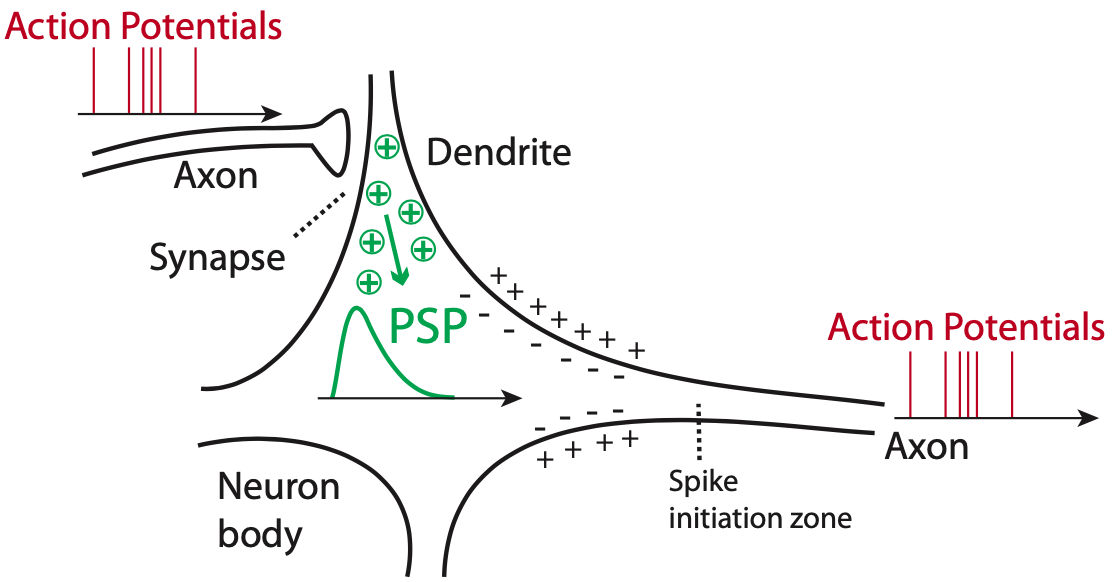
\includegraphics[scale=0.25]{pics/post-synaptic_potentials.png}
    \caption{Post-synaptic potentials in a neuron, consecutive to ion exchange}
    \source{A. \textsc{Gramfort}, MEEG course}
    \label{fig:post_synaptic_potentials}
\end{figure}

Two methods are used to capture both the electrical and the magnetic field, respectively the electroencephalography (EEG) that captures differences in electric potential at the scalp, and the magnetoencephalography (MEG) that captures magnetic flux density outside the head, as shown in Figure~\ref{fig:meeg_recordings}.
Both method record synchronised neural activity at a very high temporal resolution, about the millisecond\footnote{Sampling is often between \num{250} and \SI{1000}{\hertz}.}, and have the advantage of being non-invasive, unlike ectrocorticography (ECoG) that uses electrodes placed directly on the exposed surface of the brain.
Note that a large number of simultaneously active neurons, about \num{50000}, are needed to generate a measurable M/EEG signal\footnote{Saskia \textsc{Helbling}, \textit{What are we measuring with M/EEG?}, Goethe University Frankfurt, SPM course, May 2014}.

\begin{figure}
    \centering
    \begin{subfigure}[h]{0.45\textwidth}
        \centering
        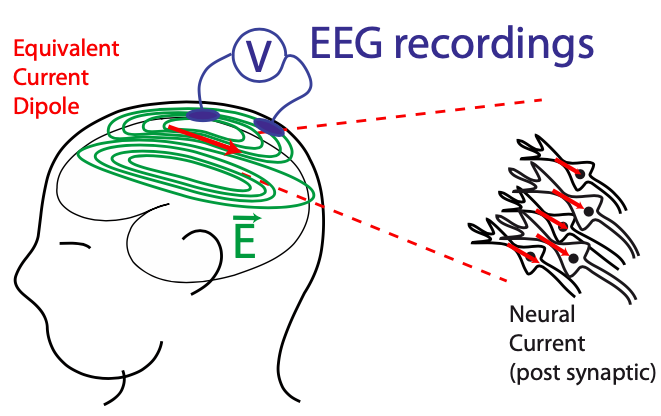
\includegraphics[width=0.9\textwidth]{pics/eeg_recordings.png}
        \caption{EEG recordings}
        \label{fig:eeg_recordings}
    \end{subfigure}
    \hfill
    \begin{subfigure}[h]{0.45\textwidth}
        \centering
        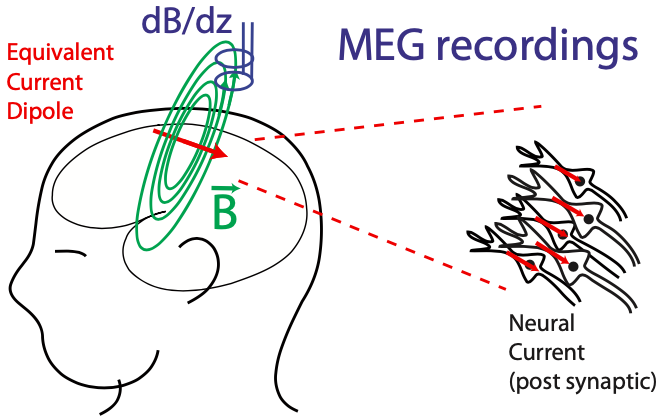
\includegraphics[width=0.9\textwidth]{pics/meg_recordings.png}
        \caption{MEG recordings}
        \label{fig:meg_recordings}
    \end{subfigure}
    \caption{Recordings of the electrical field (a) and the magnetic field (b).}
    \source{A. \textsc{Gramfort}, MEEG course}
    \label{fig:meeg_recordings}
\end{figure}

This high temporal resolution is what makes MEG and EEG attractive for the functional study of the brain.
The spatial resolution, on the contrary, is rather poor as only a few hundred simultaneous data positions can be acquired simultaneously (about \numrange{300}{400} sensors for MEG and up to \num{256} electrodes for EEG).
With appropriate models and methods, localisation of activity from MEG and EEG is nevertheless possible\footnote{\href{https://team.inria.fr/athena/fr/megeeg-vs-other-functional-brain-imaging-modalities/}{Inria: MEG/EEG vs. other functional brain imaging modalities}}.
This is what is called the \textit{inverse problem}, whose objective is to determine the current generators that produced the M/EEG measurements, as opposed to the \textit{forward problem} whose objective is to predict the M/EEG surface signal to current dipoles in the brain.

Finaly, note that neural activity recorded via M/EEG measurements is fundamental to modern experimental neuroscience and in our understanding of human cognitive processes and certain pathologies, thereby motivating the development of computational tools for learning such signals from data.
Such recordings consist of dozens to hundreds of simultaneously recorded signals, for duration going from minutes to hour \citep{jas2017learning, dupre2018multivariate}.

In this report we will mainly focus on the data recorded via MEG obtained in the course of experiments in which subjects are exposed to external stimuli.
A more comprehensive presentation of the data we work with is done in the Section~\ref{res_real_data}.
In Python, M/EEG data are easily manipulable thanks to the \href{https://mne.tools/stable/index.html}{\texttt{MNE} package} \citep{gramfort2013meg}.

\subsection{M/EEG signals decomposition via dictionary learning}\label{meeg_decomposition}

As previously explained in Section~\ref{data_in_electrophysiology}, the data recorded from one subject via M/EEG is complex.
For example, for $P$ sensors, called \textit{channels}, over $T$ timestamps, the signal observed is $X \in \R^{P\times T}$, that contains heavy noise bursts and have low signal-to-noise ratio, as most of neural signals \citep{jas2017learning}.
Thus, we cannot work directly with this result, we have to pre-process it in some way. 

It is known that neural time-series data contain a wide variety of prototypical signal waveforms (atoms) that are of significant importance in clinical and cognitive research.
One of the goals for analysing such data is hence to extract such `shift-invariant' atoms, as events can happen at any instant \citep{jas2017learning}.
While alpha waves (\SIrange{8}{12}{\hertz}) are known to closely resemble short sinusoids, and thus are revealed by Fourier analysis or wavelet transforms, there is an evolving debate that electromagnetic neural signals are composed of more complex waveforms that cannot be analysed by linear filters and traditional signal representations \cite{dupre2018multivariate}.

To learn such atoms, one method is to use \textit{dictionary learning}, that is a branch of signal processing and machine learning that aims at finding a frame (called dictionary) in which some training data admits a sparse representation.
The sparser the representation, the better the dictionary\footnote{\href{https://team.inria.fr/panama/fr/projects/please/dictionary-learning/}{Team Inria Panama - Dictionary learning: theory and algorithms}}.
Applied to brain signals, one method that works well is \textit{convolutional sparse coding} (CSC) \citep{jas2017learning, dupre2018multivariate, moreau2019distributed}.
This method aims at finding a dictionary of atoms and some associated activation vectors, in order to recover the original signal $X$ by doing a convolution between the atoms and their sparse activation vectors, as shown in Figure~\ref{fig:signal_decomposition}.

\begin{figure}[h!]
    \centering
    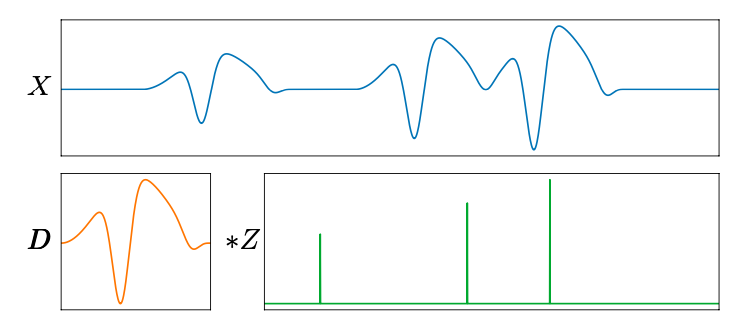
\includegraphics[scale=0.5]{pics/atom_decomposition.png}
    \caption{Decomposition of a noiseless univariate signal $X$ (blue) as the convolution $Z * \boldsymbol{D}$ between a temporal pattern $\boldsymbol{D}$ (orange) and a sparse activation signal $Z$ (green).}
    \source{\cite{moreau2019distributed}}
    \label{fig:signal_decomposition}
\end{figure}

The optimisation problem is as follow\footnote{Note that we are in the case of 1D-convolution, in multivariate CSC.}:
\begin{equation}\label{eq:csc_problem}
\begin{gathered}
\min _{D_{k}, z_{k}^{n}} \sum_{n=1}^{N} \frac{1}{2}\norme{X^{n}-\sum_{k=1}^{K} z_{k}^{n} * D_{k}}_{2}^{2}+\lambda \sum_{k=1}^{K}\norme{z_{k}^{n}}_{1} \\
\text { s.t. } \quad \norme{D_{k}}_{2}^{2} \leq 1 \text { and } z_{k}^{n} \geq 0
\end{gathered}
\end{equation}
where $\braces{X^n}_{n=1}^N \in \R^{P\times T}$ are $N$ observed multivariate signals, $\lambda > 0$ is the regularization parameter, $\braces{D_k}_{k=1}^K \in \R^{P\times L}$ are the spatio-temporal atoms, $\braces{z_k^n}_{k=1}^K \in \R^{\widetilde{T}}$ are $K$ sparse signals of activations associated with $X^n$, with $\widetilde{T} \coloneqq T - L + 1$, and where $z_{k}^{n} * D_{k}$ denotes the convolution between the two signals, obtained by by convolving every row of $D_k$ by $z_k^n$.

In order to better account for the nature of brain signals, a rank-1 constraint is added to the dictionary: $D_k = u_k v_k^T \in \R^{P\times L}$, with $u_k \in \R^P$ being the pattern over channels and $v_k \in \R^L$ over time.
Thus, the $\norme{D_{k}}_{2}^{2} \leq 1$ constraint in \eqref{eq:csc_problem} is now replaced by $\norme{u_{k}}_{2}^{2} \leq 1$ and $\norme{v_{k}}_{2}^{2} \leq 1$.
This rank-1 constraint comes from Maxwell's equations and the physical model of electrophysiological signals like EEG or MEG, where each sensor is supposed to instantly receive a linear transformation of every sources, with a constant topographic map, i.e., a signal coming from the same source at two different times will be spread across the sensors with the same linear transformation.
Thanks to this rank-1 constraint, the learned atoms have a spacial and a temporal pattern, as shown in Figure~\ref{fig:atom_location_and_form}.

\begin{figure}[h!]
    \centering
    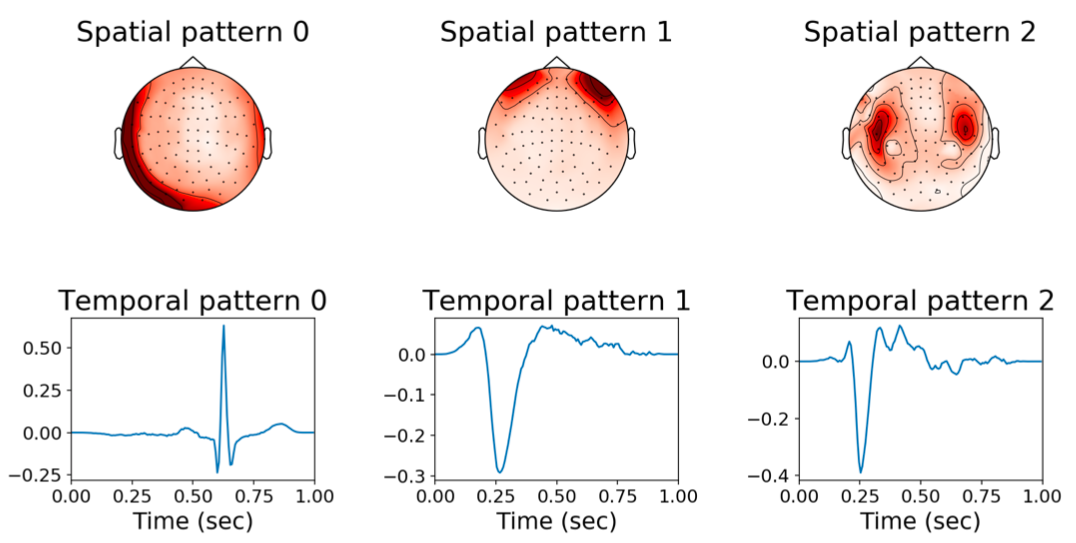
\includegraphics[scale=0.35]{pics/atom_location_and_form.png}
    \caption{Spacial (up) and temporal (down) representation of three atoms obtained by dictionary learning}
    %\source{\protect\href{https://alphacsc.github.io/auto_examples/multicsc/plot_sample_evoked_response.html#sphx-glr-auto-examples-multicsc-plot-sample-evoked-response-py}{Example in \texttt{alphacsc} package's documentation}}
    \source{Example in \texttt{alphacsc} package's documentation}
    \label{fig:atom_location_and_form}
\end{figure}

In python, the package \href{https://alphacsc.github.io/index.html}{\texttt{alphacsc}} makes it possible to carry out such an operation.
In practice, we do not have $N$ signals, as the brain of every person is different, it would make no sense to consider that the atoms of one subject are strictly identical to another.
Thus, we split the recorded signal $X\in\R^{P\times T}$ into several smaller signals, in order to take advantage of the factorised computations describe in \citep{dupre2018multivariate} that speed up computational time, and eventually to be able to distribute computations \citep{moreau2019distributed}\footnote{Note that distributed CSC is not implemented yet into \texttt{alphacsc}.}.
Once the original signal is split into $N$ smaller signals, the dictionary of atoms $D$ and their associated activations vectors $z_k^n$ are learned.
Finally, an ultimate action is done: with the learned dictionary $D$ and with the original signal $X$, the matrix $z \in \R^{K\times \widetilde{T}}$ is learned solving \eqref{eq:csc_problem}.

%\citep{jas2017learning}:
%\begin{itemize}
    %\item Neural time-series data contain a wide variety of prototypical signal waveforms (atoms) that are of significant importance in clinical and cognitive research. One of the goals for analyzing such data is hence to extract such ‘shift-invariant’ atoms.
    
    %\item convolutional sparse coding (CSC) model for learning shift-invariant atoms from raw neural signals containing potentially severe artifacts.
    
    %\item A natural way to cast the problem of learning a dictionary of shift-invariant atoms into an optimization problem is a convolutional sparse coding (CSC) approach
    
    %\item As opposed to using generic bases that have predefined shapes, such as the Fourier or the wavelet bases, these atoms provide a more meaningful representation of the data and are not restricted to narrow frequency bands.
    
    %\item neural signals often contain heavy noise bursts and have low signal-to-noise ratio.
%\end{itemize}

%Résumé de \cite{dupre2018multivariate}:
%\begin{itemize}
    %\item Frequency-specific patterns of neural activity are traditionally interpreted as sustained rhythmic oscillations, and related to cognitive mechanisms such as attention, high level visual processing or motor control. While alpha waves (8–12 Hz) are known to closely resemble short sinusoids, and thus are revealed by Fourier analysis or wavelet transforms, there is an evolving debate that electromagnetic neural signals are composed of more complex waveforms that cannot be analyzed by linear filters and traditional signal representations.
    
    %\item In this paper, we propose to learn dedicated representations of such recordings using a multivariate convolutional sparse coding (CSC) algorithm. Applied to electroencephalography (EEG) or magnetoencephalography (MEG) data, this method is able to learn not only prototypical temporal waveforms, but also associated spatial patterns so their origin can be localized in the brain.
    
    %\item Dictionary learning is one family of techniques, which consists in learning atoms (or patterns) that offer sparse data approximations.
    
    %\item When working with long signals in which events can happen at any instant, one idea is to learn shift-invariant atoms. They can offer better signal approximations than generic bases such as Fourier or wavelets, since they are not limited to narrow frequency bands.
    
    %\item In this study, we develop a multivariate model for CSC, using a rank-1 constraint on the atoms to account for the instantaneous spreading of an electromagnetic source over all the channels. -> Maxwell equation, thanks to the rank-1 model can be localized in the brain for clinical or cognitive neuroscience studies.
    
    %\item bien expliquer l'hypothèse de rang 1, comme quoi c'est une conséquence de la linéarité et de l'immédiateté des équations de Maxwell. Pour un capteur $x_n$, le signal reçu peut être représenté comme étant $S$ (l'ensemble de tous les signaux) plus un signal $v_k$ (issu d'un dipole dans le cerveau, ici intervient l'immédiateté du signal, il n'y a pas de latence) multiplié par une constante $u_{n,k}$ (ici intervient la linéarité, tous les capteurs reçoivent en même temps le même signal magnétique, à une transformation linéaire près). Ainsi, puisque l'on peut faire de même avec tous les capteurs, on peut représenter les signaux reçu comme étant $X = S + u_k v_k^T$, et ainsi on trouve que $X = \sum_k u_k v_k^T$ (le tout multiplié par un $z_k$, qui lui détermine l'activation dans le temps)
%\end{itemize}
\subsection{Background on point processes}\label{background_tpp}

In this section, we will give a short introduction on point processes, and particularly on temporal point processes with a focus on Hawkes processes.
Further details can be found in \citep{daley2003introduction, daley2007introduction}.
The sub-section~\ref{pp_definitions} comes from the PhD thesis of Massil Achab~\citep{achab2017learning}.

\subsubsection{Definitions}\label{pp_definitions}
A point process is a random element whose values are point patterns on a set $S$, a locally compact metric space equipped with its Borel $\sigma$-algebra $\mathscr{B}$.
Let $X_S$ be the set of locally finite counting measures on $S$, and $\mathcal{N}_S$ the smallest $\sigma$-algebra on $X_S$ such that all point counts ${f_B: X_s \to \N, \omega \mapsto \#\pars{\omega \cap B}}$ are measurable for $B$ relatively compact in $\mathscr{B}$, where $\# A$ denotes the cardinality of the set $A$.
A point process on $S$ is a measurable map $\xi$ from a probability space $\pars{\Omega, \mathcal{F}, \proba{}}$ to the measurable space $\pars{X_S, \mathcal{N}_S}$.

Every realisation of a point process $\xi$ can be written as $\xi = \sum_{i=1}^n \dirac_{X_i}$, where $\dirac$ is the Dirac measure, $n$ is a integer-valued random variable and $X_i$'s are random elements of $S$.
A point process can be equivalently represented by a counting process $N\pars{B} \coloneqq \integ{B}{\xi (x)}{x}$ which basically is the number of event in each Borel subset $B\in\mathscr{B}$.
The mean measure $M$ of a point process $\xi$ is a measure on $S$ that assigns to every $B\in\mathscr{B}$ the expected number of event of $\xi$ in $B$, i.e., $M\pars{B} \coloneqq \esp{N\pars{B}}$ for all $B\in\mathscr{B}$.


\subsubsection{Temporal point processes}
A temporal point process is a stochastic, or random, process composed of a time series of binary events that occur in continuous time\footnote{\href{http://www.stat.columbia.edu/~liam/teaching/neurostat-fall19/uri-eden-point-process-notes.pdf}{Liam Paninski, Statistical analysis of neural data, Fall 2019, \textit{Chapter 2: Introduction to Point Processes} - Columbia Statistics}}.
However, on the contrary of time series, temporal point processes can study multiple time scales at once~\citep{bompaire2019machine}. 

In this particular case, $S$ is the time interval $\intervalleFO{0}{T}$, equipped with the Borel $\sigma$-field of the real line $\mathscr{B}\pars{\R}$.
Here, a realisation of a point process is simply a set of time points: $\xi = \sum_{i=1}^n \delta_{t_i}$.
With a slight abuse of notation, we associate to the set of distinct random timestamps $\xi = \braces{t_1, \dots, t_n}$ occurring before $T$, the counting process $N_t = \sum_{t_i \in\xi}\1[t_i \leq t]$, which is then simply the number of points in the time interval $\intervalleOF{0}{t}$.
This counting process is a random process which evolves over time by jumps of size 1.
Studying temporal point processes consists in analysing when this jumps occur.
The \textit{conditional intensity} function $\lambda\pars{t \middle| \mathscr{F}_t}$ is the usual way to characterise temporal point processes where the present depends on the past.
It is defined as the expected infinitesimal rate at which events are expected to occur after $t$ given the information $\mathscr{F}_t$ available up to (but not including) time $t$, i.e., the history of the counting process $N_t$ prior to $t$.
Namely,
\begin{equation}
    \lambda\pars{t \middle| \mathscr{F}_t} = \lim_{\dint t \to 0} \frac{\proba{N_{t + \dint t} - N_t = 1}[\mathscr{F}_t]}{\dint t}
\end{equation}
where $\mathscr{F}_t = \enstq{t_i}{t_i < t, i=1,\dots,n}$ is the natural filtration of the process.
The conditional intensity function is sometimes denoted $\lambda^*(t)$.

As $\dint N_t \coloneqq N_{t +\dint t} - N_t \in \braces{0,1}$ can only increase by one event at each $\dint t$, it readily follows that $\proba{\dint N_t = 1}[\mathscr{F}_t] = \lambda^*(t)\dint t$ and
\begin{equation}
    \esp{\dint N_t}[\mathscr{F}_t] = 1\times \proba{\dint N_t = 1}[\mathscr{F}_t] + 0\times \proba{\dint N_t = 0}[\mathscr{F}_t] = \lambda^*(t)\dint t
\end{equation}
Hence, we can also think of the conditional intensity function $\lambda^*(t)$ as an instantaneous rate of events per time of unit.

The \textit{homogeneous Poisson process} is the most simple temporal point process, which assumes that the events arrive at a constant rate, which corresponds to a constant intensity function $\lambda\pars{t \middle| \mathscr{F}_t} = \lambda^*(t) = \lambda > 0$.
In other words, it describe a phenomenon with no memory and a constant probability of occurrence in which $N_{t + \Delta t} - N_t$ follows a Poisson distribution of parameter $\Delta t$ for any $\Delta t > 0$.
For this process, $\forall B \in \mathscr{B}\pars{\R}, M\pars{B} = \lambda \abs{B}$, where $\abs{\cdot}$ is the Lebesgue measure on $\pars{S, \mathscr{B}\pars{\R}}$.

The \textit{inhomogeneous Poisson process} is a more general process, for which the conditional intensity function is not constant as it depends on $t$ but \textit{not} on the history, i.e. $\lambda\pars{t \middle| \mathscr{F}_t} = \lambda^*(t) = \lambda(t)$.
For this process, $M\pars{B} = \integ{B}{\lambda(x)}{x}$, for all $B \in \mathscr{B}\pars{\R}$.

Let us denote $f^*(t) = f\pars{t \middle| \mathscr{F}_t}$ the conditional probability density function of the inter-event time, i.e., the probability that the next event will occur during the interval $\intervalleFO{t}{t+\dint t}$ conditioned on the history $\mathscr{F}_t$.
Let us also denote $F^*(t) = F\pars{t \middle| \mathscr{F}_t} = \proba{t_n \leq t_{n+1} \leq t}[\mathscr{F}_t] =  \integ{t_{n}}[t]{f^*(\tau)}{\tau}$ the conditional cumulative density function, i.e., the probability that the next event will occur before time $t$ conditioned on the history $\mathscr{F}_t$, where here $t_n$ is the last event in $\mathscr{F}_t$, i.e., the last event before time $t$.
Finally, we denote $S^*(t) = 1 - F^*(t) = \proba{t_{n+1} \geq t}[\mathscr{F}_t]$ the complementary cumulative distribution, also called the survival function, i.e., the probability that the next event will not occur before time $t$ conditioned on the history $\mathscr{F}_t$ \citep{de2019temporal}.
Now,
\begin{equation}
    \begin{split}
        \lambda^*(t) &= \lim_{\dint t \to 0} \frac{\proba{t\leq t_{n+1} \leq t+\dint t}[t_{n+1} > t]}{\dint t} \\
        &= \lim_{\dint t \to 0} \frac{1}{\dint t} \frac{\proba{t\leq t_{n+1} \leq t+\dint t}}{\proba{t_{n+1} > t}} \\
        &= \lim_{\dint t \to 0} \pars{\frac{1}{\dint t}\frac{f^*(t)\dint t}{S^*(t)} + o(1)} \\
        &= \frac{f^*(t)}{S^*(t)} \\
        &= - \frac{1}{S^*(t)} \deriv{S^*(t)}{t} \\
        &= -\deriv{\log S^*(t)}{t}
    \end{split}
\end{equation}
By integrating the left and right hand sides in the above equation, we have that
\begin{equation}
    \integ{t_n}[t]{\lambda^*(\tau)}{\tau} = \integ{t_n}[t]{-\deriv{\log S^*(\tau)}{\tau}}{\tau} = -\log S^*(t) + \underbrace{\log S^*(t_n)}_{=0}
\end{equation}
and thus,
\begin{equation}
    S^*(t) = \e{- \integ{t_n}[t]{\lambda^*(\tau)}{\tau}}
\end{equation}
Finally, we get that
\begin{equation}\label{eq:f_star_res}
    f^*(t) = \lambda^*(t) \e{- \integ{t_n}[t]{\lambda^*(\tau)}{\tau}}
\end{equation}

\subsubsection{Poisson process and likelihood function}

This section is taken and adapted from \citep[chap.~2, p.~19-23]{daley2003introduction} and aims to give a more in-depth presentation of the Poisson processes, with a focus on the computation of the likelihood function, as it is a crucial information for the repport.

The stationary Poisson process\footnote{What we previously called the homogeneous Poisson process.}, on the line is completely defined by the following equation, in which we use $N\intervalleOF{a_i}{b_i}$ to denote the number of events of the process falling in the half-open interval $\intervalleOF{a_i}{b_i}$ with $a_i < b_i \leq a_i+1$:
\begin{equation}\label{eq:def_stationary_pp}
    \proba{N\intervalleOF{a_i}{b_i} = n_i, i=1,\dots,k} = \prod_{i=1}^k \frac{\bracks{\lambda\pars{b_i-a_i}}^{n_i}}{n_i!}e^{-\lambda\pars{b_i-a_i}}
\end{equation}

This definition embodies three important features:
\begin{itemize}
    \item the number of points in each finite interval $\intervalleOF{a_i}{b_i}$ has a Poisson distribution of parameter $\lambda$;
    
    \item the numbers of points in disjoint intervals are independent random variables; and
    
    \item the distributions are stationary: they depend only on the lengths $b_i - a_i$ of the intervals.
\end{itemize}

The likelihood of a finite realisation of a Poisson process may be defined as the probability of obtaining the given number of observations in the observation period, times the joint conditional density for the positions of those observations, given their number.

Suppose that there are $N$ observations on $\intervalleOF{0}{T}$ at time points $t_1,\dots,t_N$. From \ref{eq:def_stationary_pp}, we can write down immediately the probability of obtaining single events in $\intervalleOF{t_i-\Delta}{t_i}$ and no points on the remaining part of $\intervalleOF{0}{T}$.
Let $A$ and $B$ be respectively those events, namely, 
$$A = \braces{N\intervalleOF{t_i-\Delta}{t_i} = 1, i=1,\dots,N}$$
and
$$B = \braces{N\intervalleOF{0}{t_{1}-\Delta} = 0, N\intervalleOF{t_N}{T} = 0, N\intervalleOF{t_i}{t_{i+1}-\Delta} = 0, i=1,\dots,N-1}$$
\begin{align*}
    \proba{A\cap B} &= \prod_{i=1}^N \pars{\lambda\Delta e^{-\lambda\Delta}} \times e^{-\lambda\pars{t_1 - \Delta}} \times e^{-\lambda\pars{T-t_N}} \times \prod_{i=1}^{N-1} e^{-\lambda\pars{t_{i+1}-\Delta-t_i}} \\
    &= \prod_{i=1}^N \pars{\lambda\Delta} \times e^{-\lambda \Delta N} \times e^{-\lambda\pars{T-N\Delta}} \\
    &= e^{-\lambda T} \prod_{i=1}^N \lambda\Delta \\
    &= \lambda^N \Delta^N e^{-\lambda T}
\end{align*}

Dividing by $\Delta^N$ and letting $\Delta \xrightarrow{} 0$, to obtain the density, we find as the required likelihood function
\begin{equation}
    L_{\intervalleOF{0}{T}}\pars{N;t_1,\dots,t_n} = \lambda^N e^{-\lambda T}
\end{equation}

We can extend this result to a Poisson process with time-varying rate $\lambda(t)$, commonly called the \textit{nonhomogeneous} or \textit{inhomogeneous} Poisson process.
The process can be defined exactly as in \ref{eq:def_stationary_pp}, ,with the quantities $\lambda\intervalleOF{a_i}{b_i} = \integ{a_i}[b_i]{\lambda}{x}$ replaced wherever they occur by quantities
$$ \Lambda\intervalleOF{a_i}{b_i} = \integ{a_i}[b_i]{\lambda(x)}{x}$$
called the \textit{compensator} of the point process.
Thus, the joint distributions are still Poisson, and the independence property still holds.
The likelihood function takes the more general form
\begin{equation}\label{eq:general_likelihood}
\begin{split}
    L_{\intervalleOF{0}{T}}\pars{N;t_1,\dots,t_n} &= e^{-\Lambda\intervalleOF{0}{T}} \prod_{i=1}^N \lambda(t_i) \\
    &= \e{-\integ{0}[T]{\lambda(t)}{t} + \sum_{i=1}^N \log \lambda(t_i)} \\
    &= \e{-\integ{0}[T]{\lambda(t)}{t} + \int_0^T \log \lambda(t)N\pars{\dint t}}
\end{split}
\end{equation}

Note that this result could also be obtained by using the Equation~\eqref{eq:f_star_res}.

\subsubsection{Hawkes processes}\label{hawkes_processes}

In this section, we give the main definitions and properties of Hawkes processes and multivariate Hawkes processes and set the notations that will be used if the in the rest of the report.
Hawkes processes~\citep{hawkes1971point, hawkes1974cluster} are temporal point processes in which the intensity depends on the process history with an excitation mechanism.
They can be understood as the equivalent of auto-regressive time series models (AR) but in continuous time.
This allows to study cross causality that might occur in one or several events series~\citep{bompaire2019machine}.

An Hawkes process is thus defined by a history dependent intensity $\lambda$ defined as follows:
\begin{equation}\label{eq:uni_hawkes_process}
    \lambda\pars{t\middle| \mathscr{F}_t} = \psi\pars{\mu + \integ{-\infty}[t]{\phi(t-s)}{N_s}}
\end{equation}
where 
\begin{equation}
    \integ{-\infty}[t]{\phi(t-s)}{N_s} = \sum_{i, t_i<t} \phi(t-t_i)
\end{equation}
The $\mu \geq 0$ is referred as the \textit{baseline intensity}\footnote{Some authors may also call it the background intensity.} and it corresponds to the exogenous intensity of the considered events.
The function $\phi(\cdot):\R^+\to\R$ is called the \textit{kernel function}, or the transfer function~\citep{chen2017multivariate}, and quantifies over time and in magnitude the influence of past events.
Note that the occurrence of each event $t_i$ increases the intensity by a certain amount, determined by the kernel, making the intensity history dependent and a stochastic process by itself \citep{de2019temporal}.
If the \textit{link function} $\psi$ on the right-hand side of Eq.~\ref{eq:uni_hawkes_process} is non-linear, then $\lambda(t)$ is the intensity of a non-linear Hawkes process~\citep{bremaud1996stability}.
In what follows, we only consider the case where $\psi$ is the identity function.

\paragraph{Multivariate Hawkes process} We can extend the univariate Hawkes process to model the interactions of $K\geq 1$ temporal point processes, called \textit{nodes}.

Namely, it models timestamps $\braces{t_k^{(i)}}_{k\geq 1}$ of nodes $i=1,\dots,K$ associated with a multivariate counting process $N_t = \bracks{N_t^{(1)}, \dots, N_t^{(K)}}$.
Note that for all nodes $i=1,\dots,K$, we still have that all of its timestamps $t_k^{(i)}$ occur in the time interval $\intervalleFF{0}{T}$.
The excitation dynamic between the nodes is encompassed by the auto-regressive structure of the conditional intensity.
For component $N_t^{(i)}$ it writes
\begin{equation}
    \lambda_i\pars{t \middle| \mathscr{F}_t} = \mu_i + \sum_{j=1}^K  \integ{-\infty}[t]{\phi_{i,j}(t-s)}{N_s^{(j)}}
\end{equation}
where $\phi_{i,j}(t)$ quantifies the excitation rate of an event of type $j$ on the arrival rate of events of type $i$ after a time lag $t$.
In general it is assumed that each kernel is causal and positive, meaning that Hawkes processes can only account for mutual excitation effects since the occurrence of some event can only increase the future arrival intensity of other events.
If the kernels are integrable, each entry of the $K\times K$ matrix ${\pars{\Phi}_{i,j} = \integ{0}[T]{\phi_{i,j}(t)}{t}}$ denotes the expected number of events of type $i$ directly triggered by an event of type $j$.

\begin{figure}[h]
    \centering
    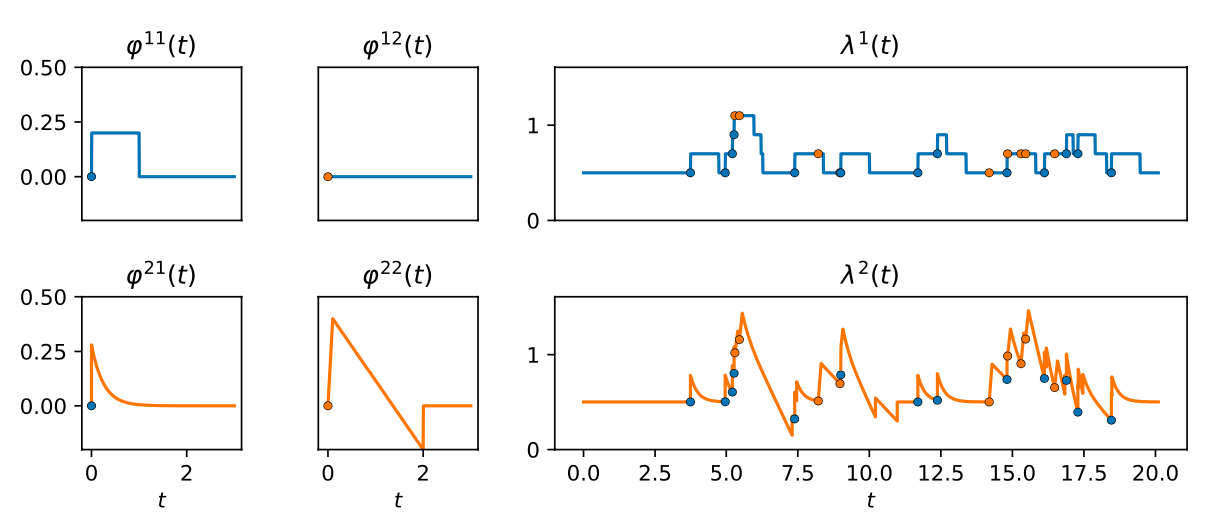
\includegraphics[scale=0.35]{pics/simu_multi_hawkes.png}
    \caption{A realisation of a 2 nodes multivariate Hawkes process. The four excitation kernels are shown on the left hand side. The intensities are displayed on the right hand side (against time, up to time 20), where events are represented by coloured dots (blue corresponding to node 1 and orange to node 2).}
    \source{\citep{bompaire2019machine}}
\end{figure}

\paragraph{Kernels parametrisation}
The main parametric model is the so-called \textit{exponential kernel}, in which the kernels have the following form:
\begin{equation}
    \phi_{i,j}(t) = \alpha_{i,j} \beta \e{-\beta t}, \quad \alpha_{i,j} > 0, \beta > 0
\end{equation}
In this model the integral matrix $\Phi = \pars{\alpha_{i,j}}_{1\leq i,j\leq K}$ and $\beta > 0$ is a memory parameter.
A more general approach is the \textit{sum of exponentials kernels}~\citep{lemonnier2014nonparametric}, namely
\begin{equation}
    \phi_{i,j}(t) = \sum_{u=1}^U \alpha_{i,j}^{(u)} \beta^{(u)} \e{-\beta^{(u)} t}, \quad \alpha_{i,j}^{(u)} > 0, \beta^{(u)} > 0
\end{equation}

Similarly, we can define the \textit{gaussian kernel} and the \textit{sum of gaussians kernels}.
In python, the \texttt{Tick} package allow to easily manipulate Hawkes process with exponential and gaussian kernels~\citep{bompaire2019machine, bacry2017tick}.
Other kernel functions are presented in~\citep{mehrdad2014hawkes}.

\section{Developed method: driven temporal point processes}\label{developed_method}

In the Hawkes processes model previously presented in Section~\ref{hawkes_processes}, the assumption is made that all the nodes might have an influence on all the other nodes, in addition of themselves.
Recall that in our application to electrophisiology, and in particular to M/EEG data, we would like to capture the potential influence of an external stimulus on the activation of a specific recurring pattern in the cortex, called \textit{atom}.
It is easy to understand in that case that the influence can only goes one way, from the stimulus process to the atom process.
Furthermore, the stimulus process is determinist as it is controlled by the experimentator and thus cannot be modeled as a classical temporal point process.
If we would like to implement such a model using \texttt{Tick}, similarly as the Figure~\ref{fig:tick_hawkes_model}, three of the four kernels would be set to the null function, as the assumption is made that the atom do not have a self-excitatory behaviour\footnote{More details on the assumptions made later in Section~\ref{hypotheses}.}, thus only leaving the kernel connecting the stimulus to the atom as a non-null function.

For those reasons, we derived a model from the Hawkes processes model, in which a determinist point process has a potential influence on a temporal point process.
By \say{having an influence on}, we mean that an event on the determinist point process increases the probability to have an event on the temporal point process.
We call this approach \textit{driven temporal point processes}, as the behaviour of a temporal point process might be driven, influenced, by a determinist point process.

\subsection{Data and notations}

TODO : Faire la distinction entre le modèle théorique (processus guidé et processus "guideur"), et l'application : les z\_k sont les processus guidés, et dans l'application on les obtient de telle manière [...] 

\begin{itemize}
    \item $\braces{z_k}_{k=1,\dots,K}$: the family of the $K$ atoms' activation vector.
    $\forall k=1,\dots,K, z_k\in\R_+^\mathbf{T}$, where $\mathbf{T}$ is the total number of possible timestamps.
    $\mathbf{T} \coloneqq T \times s_{freq}$, where $T$ is the total duration of the experimentation, and $s_{freq}$ is the sampling frequency for the collect of MEG data.
    We define $\mathcal{A}_k \coloneqq \enstq{t\times s_{freq}^{-1}}{z_k(t)\geq\tau, t=1,\dots, \mathbf{T}}$ the set of all the timestamps of atom $k$'s activations, where $\tau$ is a pre-determined threshold used to filter out insignificant activations (e.g. $\tau = \num{0.7e-10}$).
    
    \item $\braces{e_p}_{p=1,\dots,P}$: the family of the $P$ types of tasks performed during the experimentation
    \begin{equation*}
        \forall t=1,\dots,\mathbf{T}, \quad e_p(t)=
        \left\{
		\begin{array}{ll}
			1 & \mbox{if a task of type $p$ has occurred at the $t$-th timestamp}\\
			0 & \mbox{otherwise}
		\end{array}
	\right.
    \end{equation*}
    
    \item $t^{(p)} \coloneqq \enstq{t\times s_{freq}^{-1}}{e_p(t)=1, t=1,\dots, \mathbf{T}}$ denotes all the timestamps when a task of type $p$ occurred.
    We thus have $t^{(p)} = \braces{t^{(p)}_1, \dots, t^{(p)}_{n_p}}$ sorted, i.e., $t^{(p)}_1 < t^{(p)}_2 < \dots < t^{(p)}_{n_p}$, where $n_p=\# t^{(p)}$ is the total number of task $p$ that has occurred during the experimentation, as $\# A$ denotes the cardinality of the set $A$.
\end{itemize} 
\subsection{Model with truncated gaussian kernel}

TODO : partir de la forme général du kernel, avec $\phi$, comme écrit dans Hawkes, puis dire que l'on choisit un kernel normal tronqué de façon à modéliser la latency entre le stimulus et son éventuelle réponse neuronale.
Rajouter que pour l'instant on essaie de modéliser le lien entre un simulus p et un atome k, de façon à voir si ce dernier lui est lié ou non (on considère que toutes les autres influences sur l'atome k sont dans sa baseline).
Dire aussi que l'on fait l'hypothèse que, à l'inverse des processus de Hawkes avec un noyau exponentiel, où tous les events passés influent sur l'intensité présente, dans notre modèle seul le dernier event du driver à l'instant t peut avoir une influence sur l'intensité du temporal point processes qui lui est éventuellement lié (on dit toujours éventuellement cas on essaie justement d'exhiber une telle relation).

When driven by $e_p$, the dynamic of $z_k$'s counting process $N_t^{(k)} \coloneqq \sum_{t_k \in \mathcal{A}_k} \1[t_k \leq t]$ can be describe by its intensity: $\forall t\in\intervalleFF{0}{T}$,
\begin{equation}\label{eq:intensity_definition}
    \lambda_{k,p}(t) \equiv \lambda_{k}\pars{t \middle| \mathscr{F}_t^{(p)}} \coloneqq \lim_{\dint t \xrightarrow{} 0 }\frac{\proba{N_{t+\dint t}^{(k)} - N_t^{(k)} = 1}[\mathscr{F}_t^{(p)}]}{\dint t}
\end{equation}
where $\mathscr{F}_t^{(p)} = \enstq{t_i \in t^{(p)}}{t_i < t}$ is the information available on $e_p$ up to, but not including, $t$.

\paragraph{Our model}
\begin{equation}\label{eq:model_intensity}
    \lambda_{k,p}(t)  = \mu_k + \alpha_{k,p}\kappa_{k,p}(t - t_*^{(p)}(t))\1[t \geq t_1^{(p)}]
\end{equation}
where $t_*^{(p)}(t) = \max\enstq{t'}{t' \in t^{(p)}, t' \leq t}$ denotes the timestamp of the last task of type $p$ occurred before ($\leq$) time $t$, and where $\kappa_{k,p}$ is the probability density function of a truncated gaussian distribution of mean $m_{k,p}$ and standard deviation $\sigma_{k,p}$, with truncation values $\intervalleFF{a}{b}$, noted $\Norm[\bracks{a,b}]{m_{k,p}}{\sigma_{k,p}^2}$, namely,
\begin{equation}\label{eq:kernel_trunc_norm}
    \kappa_{k,p}(x) \equiv \kappa(x ; m_{k,p}, \sigma_{k,p}, a, b)=\frac{1}{\sigma_{k,p}} \frac{\phi\left(\frac{x-m_{k,p}}{\sigma_{k,p}}\right)}{\Phi\left(\frac{b-m_{k,p}}{\sigma_{k,p}}\right)-\Phi\left(\frac{a-m_{k,p}}{\sigma_{k,p}}\right)} \1[a\leq x\leq b]
\end{equation}
where
$$
\phi(x) = \frac{1}{\sqrt{2\pi}}\exp\left(-\frac{1}{2}x^2\right)
$$ 
is the probability density function of the standard normal distribution, and
$$
\Phi(x) = \frac{1}{\sqrt{2\pi}} \int_{-\infty}^x \exp\left(-\frac{1}{2}t^2\right) \mathrm{d}t
$$
is its cumulative distribution function.

Note that by definition, if $b=\infty$, then $\Phi\left(\frac{b-m_{k,p}}{\sigma_{k,p}}\right) = 1$, and similarly, if $a=-\infty$, then $\Phi\left(\frac{a-m_{k,p}}{\sigma_{k,p}}\right) = 0$.
\subsection{Hypotheses}

TODO: rapide paragraphe pour introduire les hypothèses que l'on fait, on s'inscrit quand même dans un cadre particulier lié à M/EEG

\begin{itemize}
    \item In Equation~\eqref{eq:model_intensity}, the kernel's purpose is to capture the delay of the neurological response following an external stimulation.
    This kernel is chosen to be a truncated normal of shape parameter $m$ and $\sigma$, respectively representing the mean and the standard deviation of such a delay.
    Precisely, we suppose that we have:
    \begin{equation}\label{eq:m_in_between}
        a \leq m \leq b
    \end{equation}
    where $a$ and $b$ are respectively the lower and upper truncation values.
    
    \item The shape parameters of the kernel depend on the couple atom/task, i.e. $m\equiv m_{k,p}$ and $\sigma \equiv \sigma_{k,p}$, in order to better capture the specificity of a task and its neurological response (in time and in space).
    
    \item The truncation values $a$ and $b$ are the same for every atom $k$ and every task $p$.
    The idea behind this hypothesis is that the neurological response cannot, in any case, be shorter than $a$ (e.g. $a = 50\times 10^{-3}$ second) nor be longer than $b$ (e.g. $b = 500\times 10^{-3}$ second)
    
    \item The tasks are far enough apart from each other such that the kernel is null right before every tasks, i.e.:
    \begin{equation}\label{eq:separated_timestamps}
        t_{i+1}^{(p)} - t_i^{(p)} > b, \quad \forall p=1,\dots,P, \quad \forall i=1,\dots, (n_p-1)
    \end{equation}
    In the M/EEG context, we say that the \textit{inter stimulus interval} (ISI) is larger than $b$.
    
    Note that with this hypothesis, the intensity can be rewritten similar as a auto-regressive point process:
    \begin{equation}
        \lambda_{k,p}(t)  = \mu_k + \alpha_{k,p}\sum_{t_i^{(p)} \leq t} \kappa_{k,p}(t - t_i^{(p)})
    \end{equation}
    indeed, as $t \geq t_*^{(p)}(t) > \dots > t_2^{(p)} > t_1^{(p)}$, then $\forall i, t_i^{(p)} < t_*^{(p)}(t)$
    \begin{align*}
        t - t_i^{(p)} &= t - t_{i+1}^{(p)} + t_{i+1}^{(p)} - t_i^{(p)} \\
        &> t - t_{i+1}^{(p)} + b \\
        &\geq b, \quad \text{as } t - t_{i+1}^{(p)}\geq 0
    \end{align*}
    and as by definition, $\forall x \geq b, \kappa_{k,p}(x)=0$, thus $\kappa_{k,p}(t - t_1^{(p)}) = 0$, and finally,
    \begin{align*}
        \sum_{t_i^{(p)} \leq t} \kappa_{k,p}(t - t_i^{(p)}) &= \kappa_{k,p}(t - t_1^{(p)}) + \kappa_{k,p}(t - t_2^{(p)}) + \dots + \kappa_{k,p}(t - t_*^{(p)}(t)) \\
        &= 0 + 0 + \dots + \kappa_{k,p}(t - t_*^{(p)}(t))
    \end{align*}
    
    \item The experimentation ends after every possible neurological response driven by a task, i.e.,
    \begin{equation}\label{eq:long_duration}
        \forall p=1,\dots,P, \quad T > t_{n_p}^{(p)} + b
    \end{equation}
    $$
    \Leftrightarrow T > \maxx{p=1,\dots,P} t_{n_p}^{(p)} + b
    $$
    \item An atom can be driven by only one task, but a task can drive several atoms. TODO: oui et donc ? dire que c'est pour la première version du modèle
    
    \item The baseline intensity $\mu_k$ is fixed in time.
\end{itemize}
\subsection{Simulation}

TODO: présenter pourquoi on utilise cet algorithme, citer aussi le papier pour l'algo de simulation des processus de hawkes, et redire pourquoi ce n'est pas exactement notre cas (on est déterministe sur un des processus temporel)

\cite{ogata1981lewis, chen2016thinning, lewis1979simulation}

\begin{algorithm}[htpb]
\SetKw{KwDraw}{Draw}

\SetAlgoLined
\KwData{$\lambda(t)$, $T$}

initialize $n = m = 0$, $t_0 = s_0 = 0$, $\Bar{\lambda} = \max_{0 \leq t \leq T} \lambda(t)$\;
\While{$s_m \leq T$}{
   \KwDraw $u \sim \Unif{\intervalleFF{0}{1}}$\;
   $w \leftarrow -\ln u / \Bar{\lambda}$ \atcp{so that $w\sim \Exp{\Bar{\lambda}}$}
   $s_{m+1} \leftarrow s_m + w$\;
   \KwDraw $D \sim \Unif{\intervalleFF{0}{1}}$\;
   \If{$D \leq \lambda(s_{m+1}) / \Bar{\lambda}$}{
      $t_{n+1} \leftarrow s_{m+1}$\;
      $n \leftarrow n+1$\;
      }
   $m \leftarrow m+1$\;
   }
\eIf{$t_n \leq T$}{
   \Return $\braces{t_k}_{k=1,2,\dots,n}$\;
   }{
   \Return $\braces{t_k}_{k=1,2,\dots,n-1}$\;
   }
\caption{\cite{lewis1979simulation}, p.7, Algorithm 1, One-dimensional nonhomogeneous Poisson process}\label{algo:1d_inhomogenous_pp}
\end{algorithm}

\subsection{EM-based algorithm}

As mentioned above, we would like to fit a model between an atom $k$ and a specific type of stimulus $p$ that would explain the activations of the atom, assuming that the stimulus $p$ might \say{drive} the atom $k$.
It has been hypothesised that the activations of the atom $k$, when driven by the stimulus $p$ follow a temporal point process of intensity $\lambda_{k,p}$ as described in Equation~\eqref{eq:model_intensity}.
To \say{fit} the model simply means that we need to find optimal values of the parameters of the intensity, namely $\mu_k, \alpha_{k,p}, m_{k,p}$ and $\sigma_{k,p}$, that minimise a certain metric, namely the negative log-likelihood.
A way to find such optimal values is by doing a EM-based algorithm, inspired by such algorithm described in \citep{lewis2011nonparametric, xu2016learning} for similar problematic but with different approaches (Hawkes processes, exponential kernels, etc.).

Computations of such an algorithm are detailed below, after a rewriting a the kernel formula, in order to simplify further computations.
In addition, we present later on in Section~\ref{parameters_initialisation} two methods to initialise the parameters, a random one and a \say{smart} one.

\subsubsection{Computations of the coefficients update}

\paragraph{Rewriting of the kernel $\kappa$}
\begin{align*}
    \kappa(x ; m, \sigma, a, b) &= \frac{1}{\sigma} \frac{\phi\pars{\frac{x-m}{\sigma}}}{\Phi\pars{\frac{b-m}{\sigma}} - \Phi\pars{\frac{a-m}{\sigma}}} \1[a\leq x\leq b] \\
    &= \frac{1}{\sigma} \frac{\e{-\frac{1}{2} \frac{\pars{x-m}^2}{\sigma^2}}}{\integ{\frac{a-m}{\sigma}}[\frac{b-m}{\sigma}]{\e{\frac{-t^2}{2}}}{t}} \1[a\leq x\leq b] \\
    &= \frac{\e{-\frac{1}{2}\frac{\pars{x-m}^2}{\sigma^2}}}{\integ{a}[b]{\e{-\frac{1}{2}\frac{\pars{u-m}^2}{\sigma^2}}}{u}} \1[a\leq x\leq b], \quad t = \frac{u-m}{\sigma} \\
    &= \frac{\e{-\frac{1}{2}\frac{\pars{x-m}^2}{\sigma^2}}}{C\pars{m,\sigma,a,b}} \1[a\leq x\leq b]
\end{align*}
where 
\begin{align*}
    C\pars{m,\sigma,a,b} &\coloneqq \integ{a}[b]{\e{-\frac{1}{2}\frac{\pars{u-m}^2}{\sigma^2}}}{u} \\
    &= \sigma\sqrt{2\pi}\pars{\Phi\pars{\frac{b-m}{\sigma}} - \Phi\pars{\frac{a-m}{\sigma}}}
\end{align*}
and similarly, we denote by subscripts the partials derivatives:
\begin{align*}
    C_m\pars{m,\sigma,a,b} &\coloneqq \partiald{}{m} C\pars{m,\sigma,a,b} \\
    &= \integ{a}[b]{\frac{u-m}{\sigma^2}\e{-\frac{1}{2}\frac{\pars{u-m}^2}{\sigma^2}}}{u} \\
    &= \bracks{-\e{-\frac{1}{2}\frac{\pars{u-m}^2}{\sigma^2}}}_{a}^b \\
    &= \e{-\frac{1}{2}\frac{\pars{a-m}^2}{\sigma^2}} - \e{-\frac{1}{2}\frac{\pars{b-m}^2}{\sigma^2}}
\end{align*}
and 
\begin{align*}
    C_\sigma\pars{m,\sigma,a,b} &\coloneqq \partiald{}{\sigma} C\pars{m,\sigma,a,b} \\
    &= \integ{a}[b]{\frac{(u-m)^2}{\sigma^3}\e{-\frac{1}{2}\frac{\pars{u-m}^2}{\sigma^2}}}{u} \\
    &= \bracks{-\frac{u-m}{\sigma}\e{-\frac{\pars{u-m}^2}{2\sigma^2}}}_{a}^b + \frac{1}{\sigma} \integ{a}[b]{\e{-\frac{1}{2}\frac{\pars{u-m}^2}{\sigma^2}}}{u} \\
    &= \frac{a-m}{\sigma}\e{-\frac{\pars{a-m}^2}{2\sigma^2}} - \frac{b-m}{\sigma}\e{-\frac{\pars{b-m}^2}{2\sigma^2}} + \frac{1}{\sigma}C\pars{m,\sigma,a,b}
\end{align*}

\paragraph{Negative log-likelihood}
From Equation~\eqref{eq:general_likelihood}, we can define the negative log-likelihood adapted for our specific problem:
\begin{equation}
    \mathcal{L}_{k,p}\pars{\mu_k, \alpha_{k,p}, m_{k,p}, \sigma_{k,p}} \coloneqq -\log L\left(\lambda_k, \mathscr{F}_{T}^{(p)}\right) = \int_{0}^{T} \lambda_{k,p}(s) \mathrm{d} s-\sum_{t\in\mathcal{A}_k} \log \lambda_{k,p}(t)
\end{equation}

Hypothesis \eqref{eq:separated_timestamps} implies that $\forall i=1,\dots,n_p - 1$,
\begin{align*}
    \integ{t_i^{(p)}}[t_{i+1}^{(p)}]{\kappa_{k,p}(s - t_*^{(p)}(s))\1[s \geq t_1^{(p)}]}{s} &= \underbrace{\integ{t_i^{(p)}}[t_i^{(p)}+a]{\kappa_{k,p}(s - t_i^{(p)})}{s}}_{=0} + \underbrace{\integ{t_i^{(p)}+a}[t_i^{(p)}+b]{\kappa_{k,p}(s - t_i^{(p)})}{s}}_{=1} \\
    &+ \underbrace{\integ{t_i^{(p)}+b}[t_{i+1}^{(p)}]{\kappa_{k,p}(s - t_i^{(p)})}{s}}_{=0} \\
    &= 1
\end{align*}
and hypothesis \eqref{eq:long_duration} implies that
\begin{align*}
    \integ{t_{n_p}^{(p)}}[T]{\kappa_{k,p}(s - t_*^{(p)}(s))\1[s \geq t_1^{(p)}]}{s} &= \underbrace{\integ{t_{n_p}^{(p)}}[t_{n_p}^{(p)} + a]{\kappa_{k,p}(s - t_{n_p}^{(p)})}{s}}_{=0} + \underbrace{\integ{t_{n_p}^{(p)}+a}[t_{n_p}^{(p)} + b]{\kappa_{k,p}(s - t_{n_p}^{(p)})}{s}}_{=1} \\
    &+ \underbrace{\integ{t_{n_p}^{(p)}+b}[T]{\kappa_{k,p}(s - t_{n_p}^{(p)})}{s}}_{=0}\\
    &= 1
\end{align*}

Thus,
\begin{align*}
    \integ{0}[T]{\lambda_{k,p}(s)}{s} &= \integ{0}[T]{\mu_k + \alpha_{k,p}\kappa_{k,p}(s - t_*^{(p)}(s))\1[s \geq t_1^{(p)}]}{s} \\
    &= \mu_k T + \alpha_{k,p}\underbrace{\integ{0}[t_1^{(p)}]{ \kappa_{k,p}(s - t_*^{(p)}(s))\1[s \geq t_1^{(p)}]}{s}}_{=0} + \alpha_{k,p}\sum_{i=1}^{n_p -1} \integ{t_i^{(p)}}[t_{i+1}^{(p)}]{\kappa_{k,p}(s - t_i^{(p)})}{s} \\
    &+ \alpha_{k,p}\integ{t_{n_p}^{(p)}}[T]{\kappa_{k,p}(s - t_{n_p}^{(p)})}{s} \\
    &= \mu_k T + \alpha_{k,p}n_p
\end{align*}

Finally,
\begin{equation}
\begin{split}
    \mathcal{L}_{k,p}\pars{\mu_k, \alpha_{k,p}, m_{k,p}, \sigma_{k,p}} &= \mu_k T + \alpha_{k,p}n_p \\
    &- \sum_{t\in\mathcal{A}_k} \log \pars{\mu_k + \alpha_{k,p}\kappa_{k,p}(t - t_*^{(p)}(t); m_{k,p}, \sigma_{k,p})\1[t \geq t_1^{(p)}]}
\end{split}
\end{equation}

% TODO : calculer la complexité du calcul de la nll, comme fait dans la thèse de Martin

Then the derivatives of the inverse log-likelihood with respect to the parameters are given by
\begin{equation}
    \partiald{}{\mu_k}\mathcal{L}_{k,p}\pars{\mu_k, \alpha_{k,p}, m_{k,p}, \sigma_{k,p}} = T - \sum_{t\in\mathcal{A}_k}\frac{1}{\lambda_{k,p}(t)}
\end{equation}

\begin{equation}
\begin{split}
    \partiald{}{\alpha_{k,p}}\mathcal{L}_{k,p}\pars{\mu_k, \alpha_{k,p}, m_{k,p}, \sigma_{k,p}} &= n_p - \sum_{t\in\mathcal{A}_k}\frac{\kappa_{k,p}(t - t_*^{(p)}(t))}{\lambda_{k,p}(t)}\1[t \geq t_1^{(p)}] \\
    &= n_p - \sum_{t\in\mathcal{A}_k, t \geq t_1^{(p)}}\frac{\kappa_{k,p}(t - t_*^{(p)}(t))}{\lambda_{k,p}(t)}
\end{split}
\end{equation}

\begin{equation}
\begin{split}
    \partiald{}{m_{k,p}}\mathcal{L}_{k,p}\pars{\mu_k, \alpha_{k,p}, m_{k,p}, \sigma_{k,p}} &= -\sum_{t\in\mathcal{A}_k}\frac{\alpha_{k,p}}{\lambda_{k,p}(t)}\partiald{}{m_{k,p}}\kappa_{k,p}(t - t_*^{(p)}(t); m_{k,p}, \sigma_{k,p}, a, b)\1[t \geq t_1^{(p)}] \\
    &= -\sum_{t\in\mathcal{A}_k, t \geq t_1^{(p)}}\frac{\alpha_{k,p}}{\lambda_{k,p}(t)}\partiald{}{m_{k,p}}\kappa_{k,p}(t - t_*^{(p)}(t); m_{k,p}, \sigma_{k,p}, a, b)
\end{split}
\end{equation}
where
\begin{equation}
    \partiald{}{m}\kappa(x ; m, \sigma, a, b) = \pars{\frac{x-m}{\sigma^2} - \frac{C_m\pars{m, \sigma,a,b}}{C\pars{m, \sigma,a,b}}}\kappa(x ; m, \sigma, a, b)
\end{equation}

\begin{equation}
\begin{split}
    \partiald{}{\sigma_{k,p}}\mathcal{L}_{k,p}\pars{\mu_k, \alpha_{k,p}, m_{k,p}, \sigma_{k,p}} &= -\sum_{t\in\mathcal{A}_k}\frac{\alpha_{k,p}}{\lambda_{k,p}(t)}\partiald{}{\sigma_{k,p}}\kappa_{k,p}(t - t_*^{(p)}(t); m_{k,p}, \sigma_{k,p}, a, b)\1[t \geq t_1^{(p)}] \\
    &= -\sum_{t\in\mathcal{A}_k, t \geq t_1^{(p)}}\frac{\alpha_{k,p}}{\lambda_{k,p}(t)}\partiald{}{\sigma_{k,p}}\kappa_{k,p}(t - t_*^{(p)}(t); m_{k,p}, \sigma_{k,p}, a, b)
\end{split}
\end{equation}
where
\begin{equation}
    \partiald{}{\sigma}\kappa(x ; m, \sigma, a, b) = \pars{\frac{(x-m)^2}{\sigma^3} - \frac{C_\sigma\pars{m, \sigma,a,b}}{C\pars{m, \sigma,a,b}}}\kappa(x ; m, \sigma, a, b)
\end{equation}

To lighten notations, we define $\mathcal{A}_{k,p} = \enstq{t}{t\in\mathcal{A}_k, t \geq t_1^{(p)}}$ as the set of atom $k$'s activation timestamps that occur after the first timestamps of task $p$.
In other words, $\mathcal{A}_{k,p}$ is the set of all atom $k$'s activations that might have been driven by a task of type $p$.

\paragraph{Expectation step}
Let $P_{t,k}$ be the probability that the activation at time $t$ has been triggered by the baseline intensity of atom $k$, and $P_{t,p}$ be that probability that the activation at time $t$ has been triggered by the driver $p$ (the task $p$ in our case).
\begin{equation}
    P_{t,k} = \frac{\mu_k}{\lambda_{k,p}(t)}
\end{equation}
\begin{equation}
    P_{t,p} = \frac{\alpha_{k,p}\kappa_{k,p}\pars{t - t_*^{(p)}(t)}}{\lambda_{k,p}(t)}\1[t \geq t_1^{(p)}]
\end{equation}

\paragraph{Maximisation step} 
In the following, we denote with the upper script the iteration step, e.g., $\theta^{(n)}$ is the value of the parameter $\theta$ at step $n$ of the EM algorithm.
By extension, if $f$ is a function of $\theta_1, \dots, \theta_m$, then we define $f^{(n)}\pars{\theta_1, \dots, \theta_m} \coloneqq f\pars{\theta_1^{(n)}, \dots, \theta_m^{(n)}}$.
Details of the computation are present in Appendix~\ref{annexe:details_em}.

\begin{equation}
    \mu_k^{(n+1)} = \frac{1}{T} \sum_{t\in\mathcal{A}_k} P_{t,k}^{(n)}
\end{equation}

\begin{equation}
    \alpha_{k,p}^{(n+1)} = \frac{1}{n_p} \sum_{t\in\mathcal{A}_{k,p}} P_{t,p}^{(n)}
\end{equation}

\begin{equation}
    m_{k,p}^{(n+1)} = \frac{\sum_{t\in\mathcal{A}_{k,p}} \pars{t - t_*^{(p)}(t)} P_{t,p}^{(n)}}{\sum_{t\in\mathcal{A}_{k,p}} P_{t,p}^{(n)}} - {\sigma_{k,p}^{(n)}}^2 \frac{C_m\pars{m_{k,p}^{(n)}, \sigma_{k,p}^{(n)},a,b}}{C\pars{m_{k,p}^{(n)}, \sigma_{k,p}^{(n)},a,b}}
\end{equation}

\begin{equation}
    \sigma_{k,p}^{(n+1)} = \pars{\frac{C\pars{m_{k,p}^{(n)}, \sigma_{k,p}^{(n)},a,b}}{C_\sigma\pars{m_{k,p}^{(n)}, \sigma_{k,p}^{(n)},a,b}} \frac{\sum_{t\in\mathcal{A}_{k,p}} \pars{t - t_*^{(p)}(t) - m_{k,p}}^2 P_{t,p}^{(n)}}{\sum_{t\in\mathcal{A}_{k,p}}  P_{t,p}^{(n)}}}^{1/3}
\end{equation}

\paragraph{Remark} If $\alpha_{k,p} = 0$, then the intensity is reduced to its baseline, $\lambda_{k,p}(t) = \mu_k$, and then the negative log-likelihood is:
\begin{equation}
    \mathcal{L}_{k,p}\pars{\mu_k, \alpha_{k,p}, m_{k,p}, \sigma_{k,p}} = \mu_k T -\sum_{t\in\mathcal{A}_k} \log \mu_k = \mu_k T - \#\mathcal{A}_k \log \mu_k
\end{equation}
Thus, we can directly compute the maximum likelihood estimator (MLE) for $\mu_k$, as follow:
\begin{equation}
    \mu_k^{(MLE)} = \frac{\#\mathcal{A}_k}{T}
\end{equation}
Note that in that case, we are no longer interested in the possible values of $m_{k,p}$ and $\sigma_{k,p}$.

\subsubsection{Parameters initialisation}\label{parameters_initialisation}

In this section, we will describe two methods on how to initialise the parameters for the EM algorithm, in other words, how to determine $\theta^{(0)} = \pars{\mu^{(0)}, \alpha^{(0), }m^{(0)}, \sigma^{(0)}}$.
\paragraph{Random initialisation}
The first initialisation method is simply done by random sampling the parameters according to a specific uniform distribution:
\begin{itemize}
    \item $\mu^{(0)} \sim \Unif{\intervalleFF{\mu_{min}}{\mu_{max}}}$, e.g. $\mu_{min} = 0.1$ and $\mu_{max} = 5$;
    
    \item $\alpha^{(0)} \sim \Unif{\intervalleFF{\alpha_{min}}{\alpha_{max}}}$, e.g. $\alpha_{min} = 0.1$ and $\alpha_{max} = 5$;
    
    \item $m^{(0)} \sim \Unif{\intervalleFF{a}{b}}$, were $a$ and $b$ are the truncation values of the kernel, Eq.~\eqref{eq:kernel_trunc_norm};
    
    \item $\sigma^{(0)} \sim \Unif{\intervalleFF{\sigma_{min}}{\sigma_{max}}}$, e.g. $\sigma_{min} = 0.01$ and $\sigma_{max} = 1$.
\end{itemize}

\paragraph{Smart initialisation}
Another method, more intuitive, would be to compute the empirical values of those parameters.
We call this method \say{smart initialisation}.
More specifically, the initial values of the parameters are computed as follow:
\begin{itemize}
     \item Let $\mathcal{D}_{k,p} \coloneqq \enstq{t-t_*^{(p)}(t)}{t\in\mathcal{A}_{k,p}} \cap \intervalleFF{a}{b}$ be the set of all empirical delays possibly linked to the task $p$.
    Then, we define $m^{(0)}$ as the mean of the empirical delays:
    \begin{equation}
        m^{(0)} = \frac{1}{\#\mathcal{D}_{k,p}}\sum_{d \in \mathcal{D}_{k,p}} d
    \end{equation}
    where $\# A$ denotes the cardinality of the set $A$.
    
    \item Similarly, we define $\sigma^{(0)}$ as the standard deviation of the empirical delays:
    \begin{equation}
        \sigma^{(0)} = \sqrt{\frac{1}{\#\mathcal{D}_{k,p}}\sum_{d \in \mathcal{D}_{k,p}} \abs{d - m^{(0)}}^2}
    \end{equation}
    
    \item The activations that do not lend on any kernel support come from the baseline intensity, which is fixed, so it is similar to say that those activations are the result of a homogeneous Poisson process.
    Thus, to initialise the baseline value $\mu^{(0)}$, we simply compute the Poisson process parameter's estimator, which is the average number of activation over the process' duration:
    \begin{equation}\label{eq:baseline_init}
    \begin{split}
        \mu^{(0)} &= \frac{\#\braces{\mathcal{A}_k \setminus \enstq{t}{t\in\mathcal{A}_{k,p}, a\leq t-t_*^{(p)}(t)\leq b}}}{T - n_p\pars{b-a}} \\
        &= \frac{\#\mathcal{A}_k - \#\enstq{t}{t\in\mathcal{A}_{k,p}, a\leq t-t_*^{(p)}(t)\leq b}}{T- n_p\pars{b-a}}
    \end{split}
    \end{equation}
    because there can be no duplicates, and where $n_p\pars{b-a}$ is the sum of all kernels support.
    
    \item Finally, we set $\alpha^{(0)}$ as follow:
    \begin{equation}
    \alpha^{(0)} = f(p_a)
    \end{equation}
    with
    \begin{equation}
        f(p_a) = - e^{\mu} \ln\pars{\frac{l(\mu) - p_a}{l(\mu)  - p_s}}
    \end{equation}
    and
    \begin{equation}
        l(\mu) = \pars{\frac{e^{\mu}-1}{5} + \frac{1}{1-p_s}}^{-1} + p_s
    \end{equation}
    where
    \begin{equation}
        p_a \coloneqq \frac{\#\enstq{t}{t\in\mathcal{A}_{k,p}, a\leq t-t_*^{(p)}(t)\leq b}}{\#\mathcal{A}_k}
    \end{equation}
    is the proportion of activations that lend in a kernel support, and 
    \begin{equation}
        p_s \coloneqq \frac{n_p\pars{b-a}}{T}
    \end{equation}
    is the ratio of all the kernels' support time over the total duration.
    
    More details on the role of the $\alpha$ coefficient and how its initialisation function was determined are presented in Appendix~\ref{app:role_alpha_coef}.
    
\end{itemize}





\subsection{Model extension to multiple point processes drivers}\label{model_extension_multiple_pp}

In the above, the model presented considered only one potential \say{driver}, as for every atom, the intensity $\lambda_{k,p}$ was only influenced by the stimulus $p$.
However, this assumption may be somewhat too restrictive.
Indeed, it is quite possible that an atom $k$ to be stimulated by both stimuli $p$ and $p'$ at the same time.
A first solution simply consists in combining both $p$ and $p'$ timestamps by defining $t^{(p, p')} \coloneqq t^{(p)} \cup t^{(p')}$, and thus,
\begin{equation}\label{eq:intensity_combined_stimuli}
    \lambda_{k,(p, p')}(t)  = \mu_k + \alpha_{k,(p, p')}\kappa_{k,(p, p')}(t - t_*^{(p, p')}(t))\1[t \geq t_1^{(p, p')}]
\end{equation}
This is this straightforward solution that is used in this work, and can easily be generalised to 3 or more \say{drivers}.

However, the main flaw of this solution is that it blurs the individual effect of each stimulus on the considered atom.
That is why when this solution is used, it is with done with stimuli that lead to similar reactions in the brain, such as two auditory stimuli, one on the left ear and the other on the right ear.
A proposed solution, which it will be interesting to deal with more in depth in future work, is to take into the intensity function multiple \say{drivers} while keeping them separated in order to be able to distinguish their respective effect on the intensity, by no longer having a single coefficient $\alpha$ for this purpose.
Let $\mathcal{P}$ be a (non-empty) set a drivers, e.g. $\mathcal{P} = \braces{p, p'}$, thus, the new intensity function can be written as follow:
\begin{equation}
    \lambda_{k,\mathcal{P}}(t)  = \mu_k + \sum_{p\in\mathcal{P}} \alpha_{k,p}\kappa_{k,p}(t - t_*^{(p)}(t))\1[t \geq t_1^{(p)}]
\end{equation}

It is possible to go even further by considering that the considered atom might eventually be influenced by the activation of other atoms, while keeping the assumption that it does not have a self-excitatory behaviour.
Hence, the intensity function must include terms for such an influence.
Let $\mathcal{K}$ be a (non-empty) set of atoms, thus, the new intensity function can be written as follow:
\begin{equation}
    \lambda_{k,\mathcal{K},\mathcal{P}}(t)  = \mu_k + \sum_{p\in\mathcal{P}} \alpha_{k,p}\kappa_{k,p}(t - t_*^{(p)}(t))\1[t \geq t_1^{(p)}] + \sum_{k'\in\mathcal{K}, k' \ne k} \beta_{k,k'} \varphi_{k,k'}\pars{t - \mathcal{A}_{k'}^*(t)}
\end{equation}
where $\mathcal{A}_{k'}^*(t) \coloneqq \max\enstq{t'}{t' \in \mathcal{A}_{k'}, t' \leq t}$ denotes the timestamp of the last activation on atom $k'$ at time $t$, $\beta_{k,k'}\in\R$ a coefficient taht allow to quantify the influence of atom $k'$ on atom $k$, and where $\varphi_{k,k'}$ is a kernel function to be specified.
Note that the final idea is that $\mathcal{P}$ and $\mathcal{K}$ are the entire set of stimuli and atoms, respectively.

The assumption of no self-excitatory behaviour can also be easily waived, thus the intensity function is only slightly modified, as follow:
\begin{equation}
    \lambda_{k,\mathcal{K},\mathcal{P}}(t)  = \mu_k + \sum_{p\in\mathcal{P}} \alpha_{k,p}\kappa_{k,p}(t - t_*^{(p)}(t))\1[t \geq t_1^{(p)}] + \sum_{k'\in\mathcal{K}} \beta_{k,k'} \varphi_{k,k'}\pars{t - \mathcal{A}_{k'}^*(t)}
\end{equation}
Note that in that case, if $k\in\mathcal{K}$, then the kernel $\varphi_{k,k}$ characterises this newly self-excitatory behaviour.

As mentioned, those new approaches are not developed nor used later on in this report and will be the subject of future work.
We only introduced them for the sake of completeness.

\section{Results}

In this section, we will present several results of interest in order to show the performances of the EM based algorithm, on both simulated and real data.
For the sake of brevity, some other figures are presented in Appendix~\ref{annexe:extra_results}.


\subsection{Simulated data}

TODO: Performances de l'algorithme EM sur des données simulées.
Parler des différents hyper-paramètres liés à l'algorithme EM, et les paramètres que l'on essaie de retrouver
\subsection{Real data}\label{res_real_data}

In this section, the results that will be presented are obtained on real data.
The main dataset that we will be using is called \textit{sample}, as it simply is the sample data available on the \texttt{MNE} package.
In this experiment, checkerboard patterns were presented to the subject into the left and right visual field, interspersed by tones to the left or right ear.
The interval between the stimuli was 750 ms.
Occasionally a smiley face was presented at the centre of the visual field.
The subject was asked to press a key with the right index finger as soon as possible after the appearance of the face\footnote{Source: \href{https://mne.tools/0.11/manual/datasets_index.html}{MNE documentation}}.
In the following, we are only interested in the four main stimuli types: auditory left, auditory right, visual left and visual right.
The experiment lasts about \SI{4.6}{\minute} and approximately 70 stimuli per type was presented, with a minimum of \SI{2.5}{\second} between two stimuli  of the same type.

As previously explained, the recorded signals must first of all be decomposed in $K$ atoms.
In our case, we put $K=40$, and some examples of obtained atoms were presented in Figure~\ref{fig:atom_location_and_form}.

Unlike the previous section where the data were simulated and thus the real values of the parameters were known, now we do not have any ground truth to compare our results to.
Thus, we will focus on showing that the algorithm converges on real data too.
However, with some domain expertise, one is able to determine the origin of a given atom.
For example, the atom 0 in Figure~\ref{fig:atom_location_and_form}, the one on the left, is characteristic of an heartbeat, which is confirmed by its spatial pattern which represents a diffuse area rather than a specific zone, as the heartbeat comes from \say{under} the brain, approximately form the middle left.
Similarly, the atom 1, the one in the middle, can easily be associated with the subject's eye blinks.
Thus, even if we do not have a ground truth, as we do not know which atom is linked to which stimulus, it can be said that some specific atoms are not linked to any stimulus, as it is the case with the heartbeat atom, for which it is reasonable to say that it is not influenced by any stimulus.
Note that such a statement is not as clear for the eye blinks atom, as the subject can eventually anticipate the incoming visual stimuli and therefore make an effort to not blink accordingly.

Let us first fit a model for atom 2, the one on the right in Figure~\ref{fig:atom_location_and_form}, alongside tasks 1 and 2, respectively the auditory on the left side stimulus and  the auditory on the right side stimulus.
We combine those two stimuli using the method presented in Equation~\eqref{eq:intensity_combined_stimuli}.
Combining those two stimuli make sens as it is understandable that two auditory stimuli would generate a similar activation in the brain.
This is confirmed by the atom's spatial representation, which has a certain axial symmetry.
Loss and parameters convergence are shown in Figures~\ref{fig:history_loss_atom_2_task_1_2} and~\ref{fig:history_params_atom_2_task_1_2}.

\begin{figure}[h!]
    \centering
    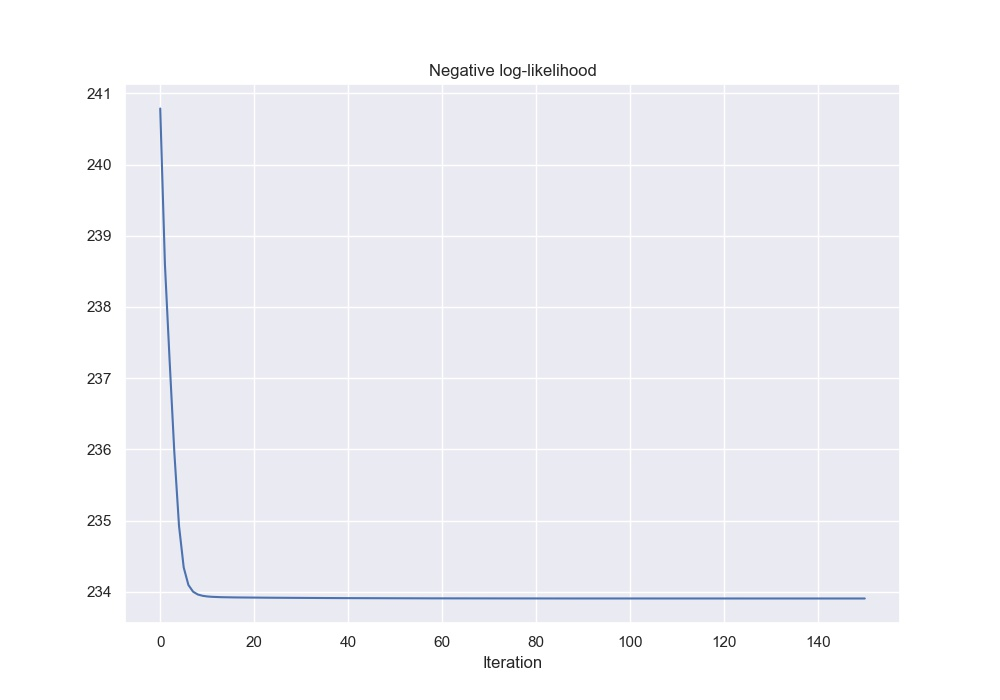
\includegraphics[width=0.9\textwidth]{pics/results_sample/history_loss_atom_2_task_1_2.jpg}
    \caption{Loss history over 150 iterations with a \textit{smart} initialisation, on sample data (atom 2, task 1 and 2) with $\intervalleFF{a}{b} = \intervalleFF{30}{800}\times \SI{e-3}{\second}$.}
    \label{fig:history_loss_atom_2_task_1_2}
\end{figure}

\begin{figure}[h!]
    \centering
    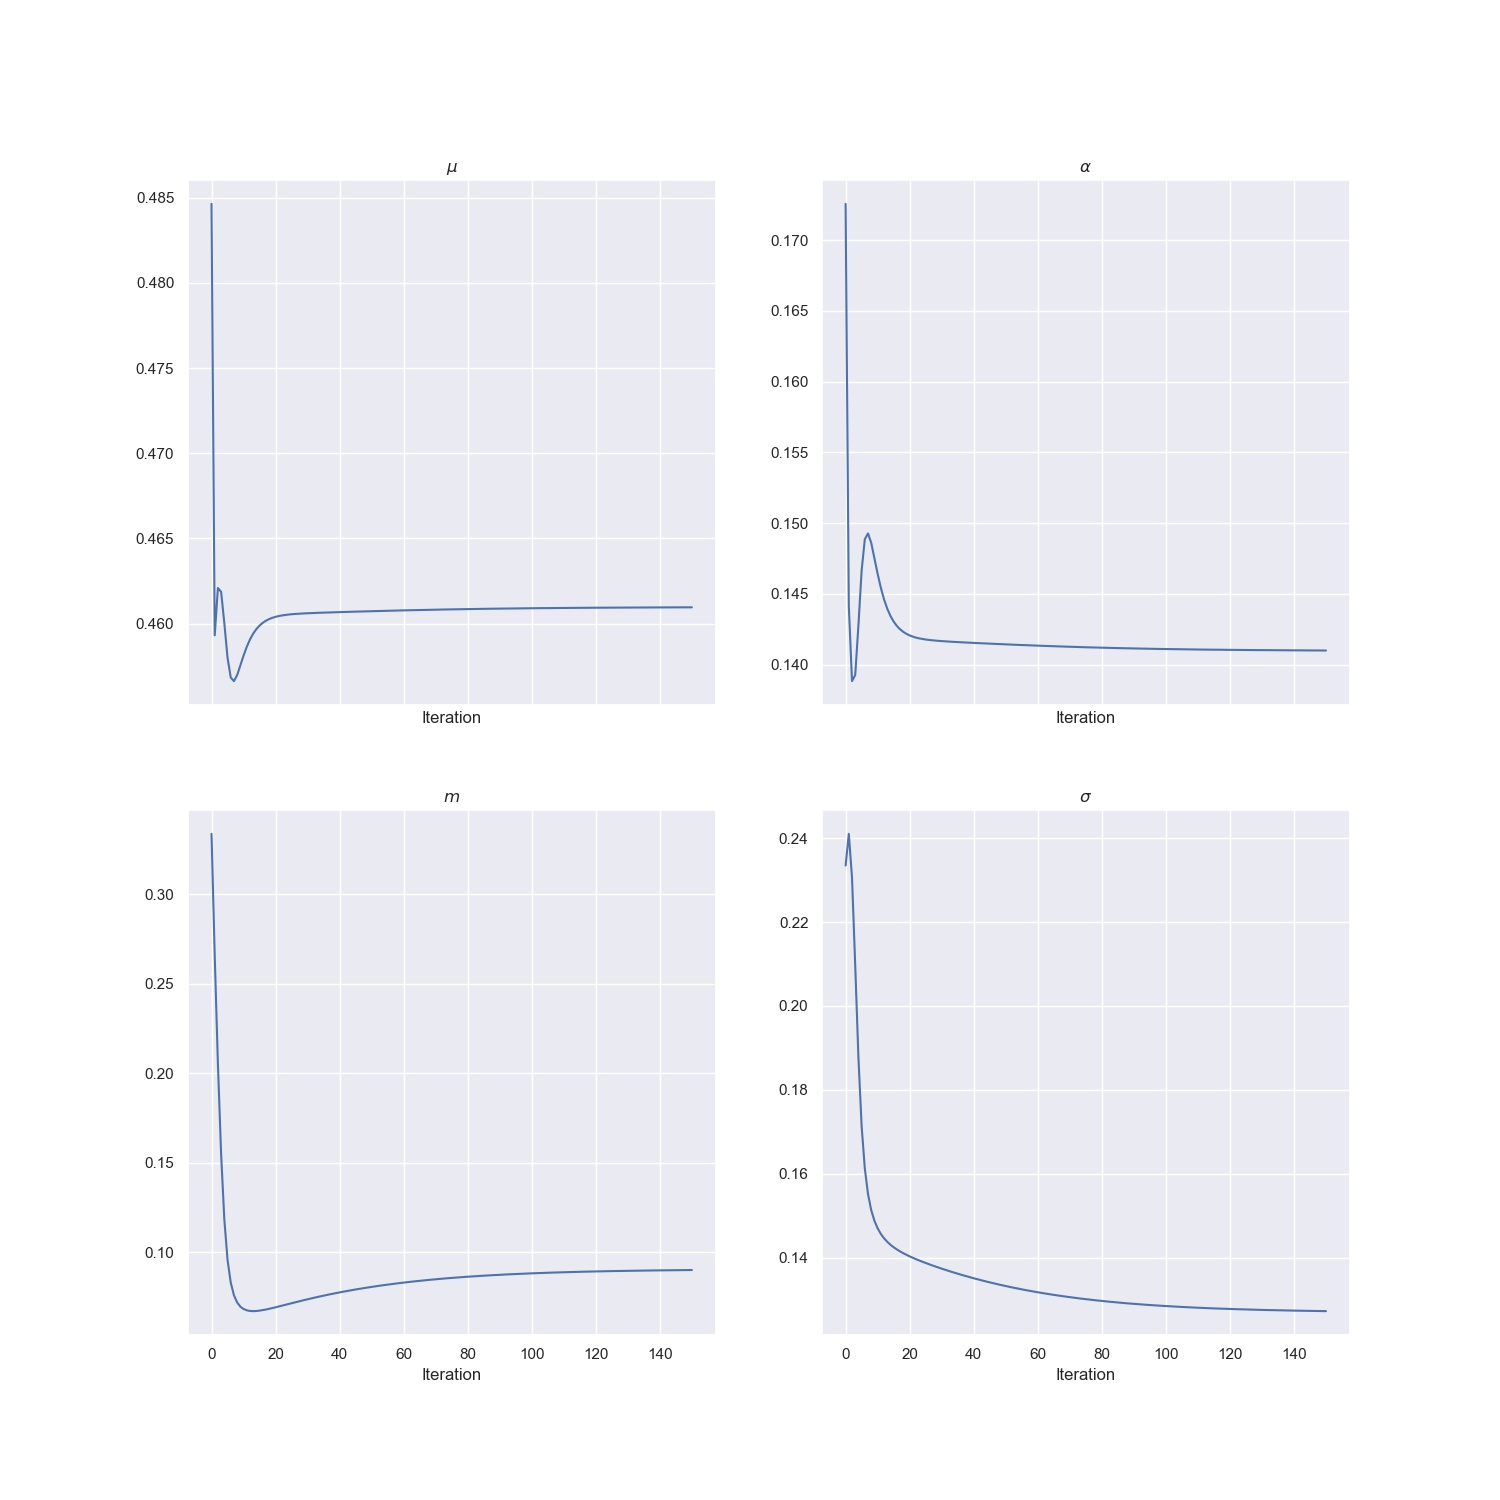
\includegraphics[width=\textwidth]{pics/results_sample/history_params_atom_2_task_1_2.jpg}
    \caption{Parameters recovery over 150 iterations with a \textit{smart} initialisation, on sample data (atom 2, task 1 and 2) with $\intervalleFF{a}{b} = \intervalleFF{30}{800}\times \SI{e-3}{\second}$.}
    \label{fig:history_params_atom_2_task_1_2}
\end{figure}

A similar experiment can be carried out on atom 0, the one that can be easily associated with a heartbeat, again alongside stimuli 1 and 2.
Loss and parameters convergence are shown in Figures~\ref{fig:history_loss_atom_0_task_1_2} and~\ref{fig:history_params_atom_0_task_1_2}.
When carried out alongside stimuli 3 and 4, respectively the visual left stimulus and the visual right stimulus, the initial value of $\alpha$ is null, thus no history is available as only the maximum likelihood estimator for the baseline parameter is computed, as mentioned in Section~\ref{parameters_initialisation}.
However, as there is no particular to consider atom 0 only alongside the auditory stimuli, one final experiment is carried out, this time by taking all of the stimuli.
Loss and parameters convergence are shown in Appendix~\ref{annexe:extra_results_real}, Figures~\ref{fig:history_loss_atom_0_task_1_2_3_4} and~\ref{fig:history_params_atom_0_task_1_2_3_4} respectively.

\begin{figure}[h!]
    \centering
    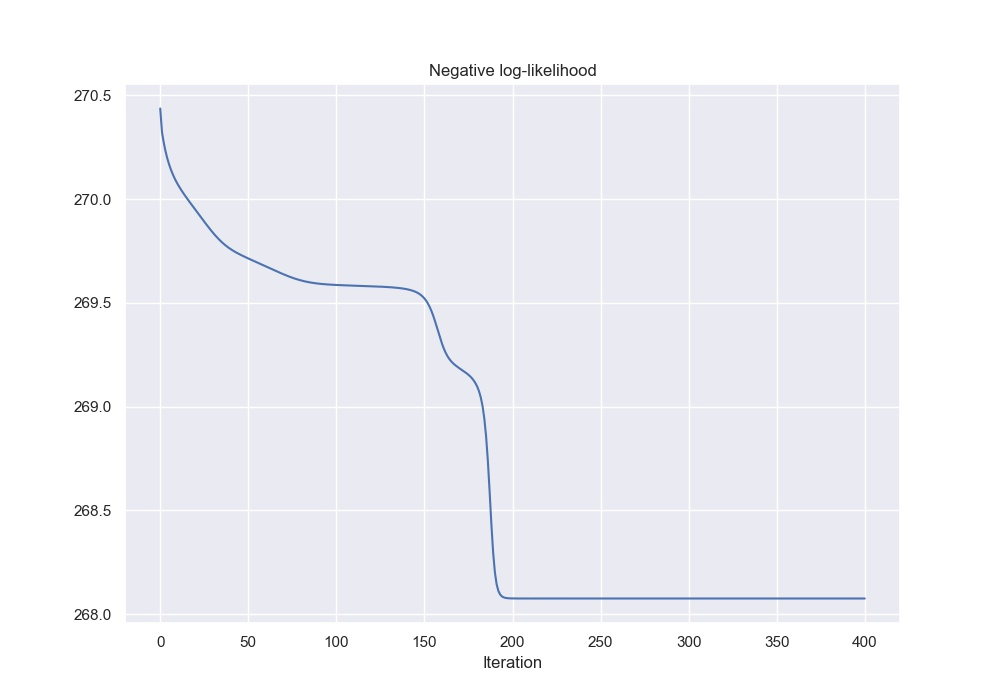
\includegraphics[width=0.9\textwidth]{pics/results_sample/history_loss_atom_0_task_1_2.jpg}
    \caption{Loss history over 400 iterations with a \textit{smart} initialisation, on sample data (atom 0, task 1 and 2) with $\intervalleFF{a}{b} = \intervalleFF{30}{800}\times \SI{e-3}{\second}$.}
    \label{fig:history_loss_atom_0_task_1_2}
\end{figure}

\begin{figure}[h!]
    \centering
    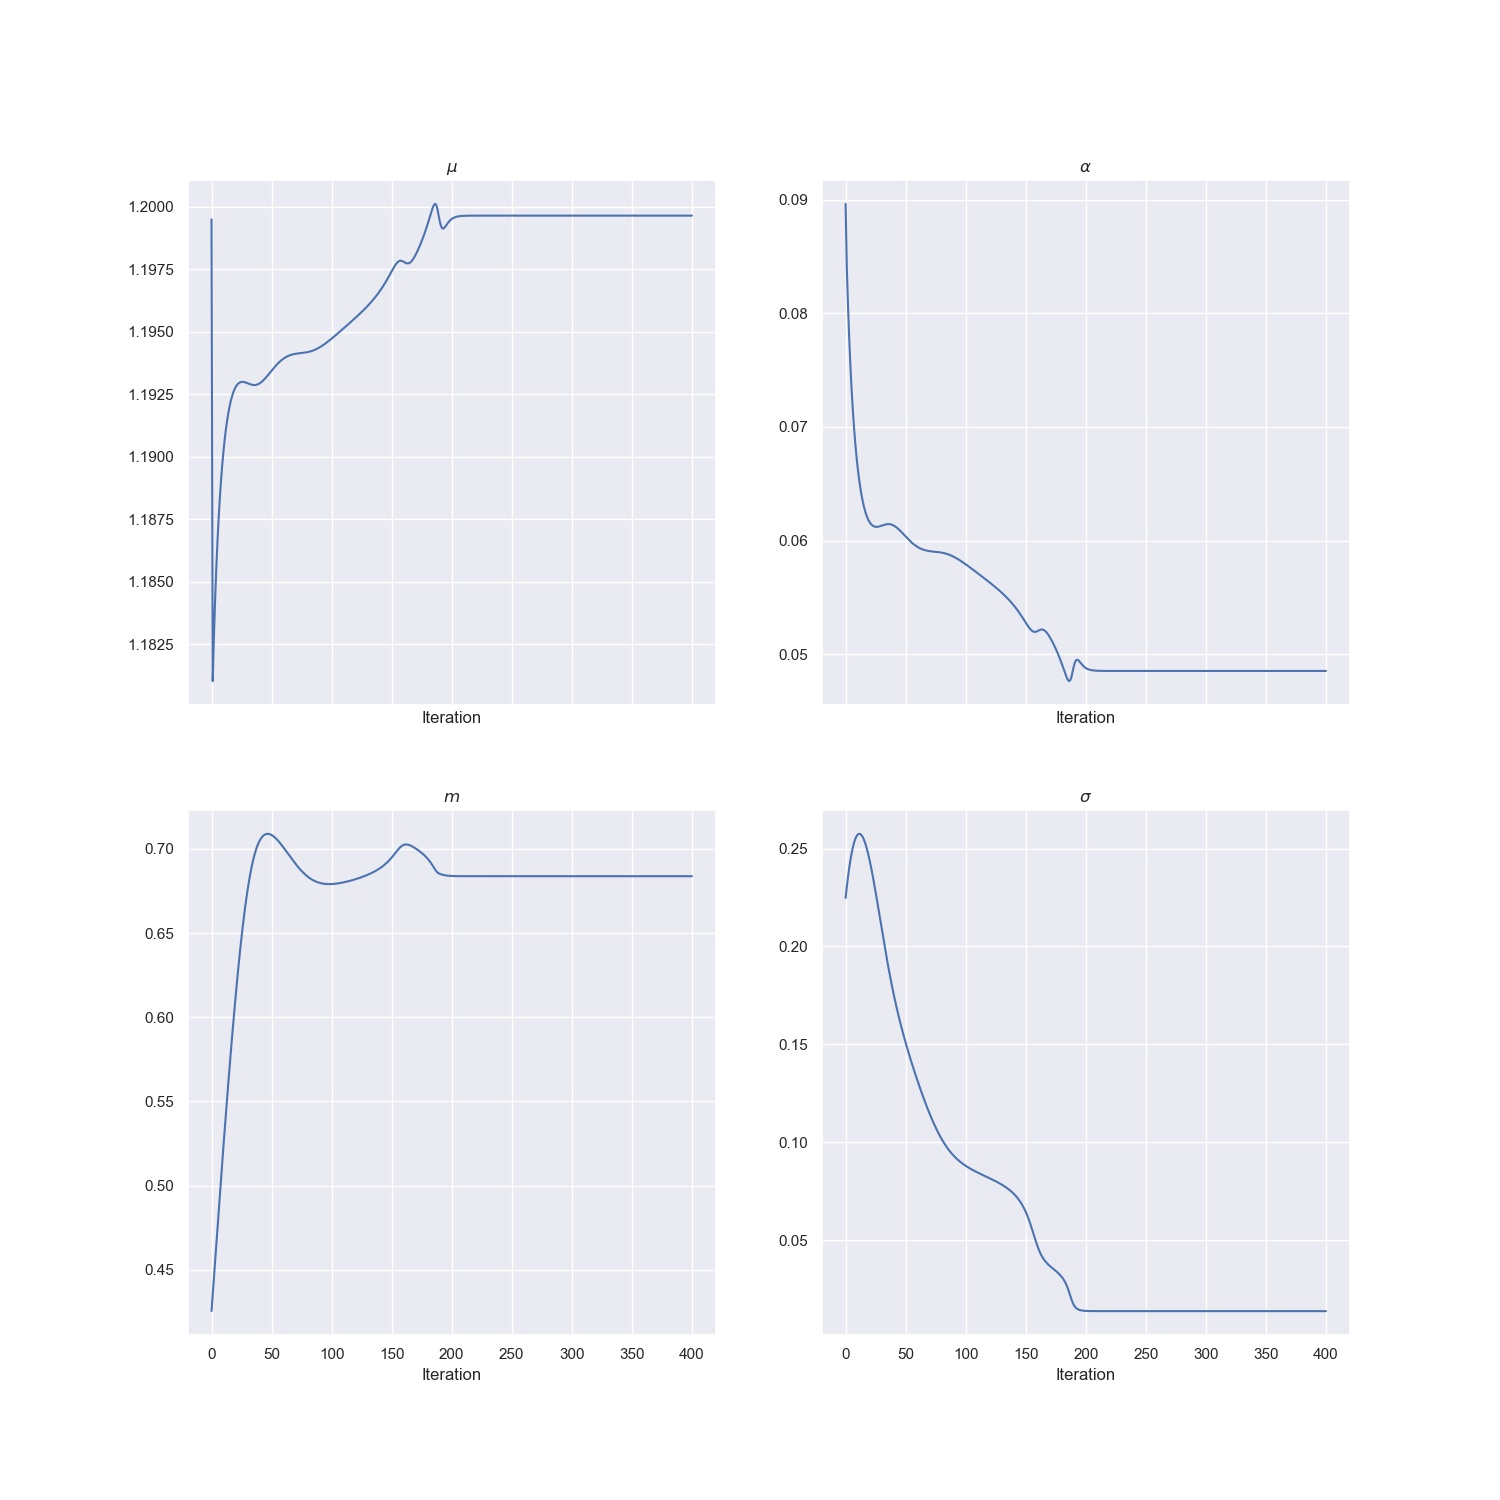
\includegraphics[width=\textwidth]{pics/results_sample/history_params_atom_0_task_1_2.jpg}
    \caption{Parameters recovery over 400 iterations with a \textit{smart} initialisation, on sample data (atom 0, task 1 and 2) with $\intervalleFF{a}{b} = \intervalleFF{30}{800}\times \SI{e-3}{\second}$.}
    \label{fig:history_params_atom_0_task_1_2}
\end{figure}

% TODO: Dire que si on connaît déjà le lien possible, on peut interpréter les résultats, parler de la mesure ration p\_a/p\_s. exemple sur sample de l'atoms lié aux battements de coeurs, qui par définition, ne doit pas avoir de lien avec aucun des task



\section{Discussion and future work}

TODO: discuss results.
Futur work: say that we know need a statistical test to determine whether or not an atom is linked to a stimulus, based on the model fitted; in alphacsc add a feature to give in input the timestamps of interest, i.e., where we are interested in finding correlated atoms; les algos convergent bien dans les différents cas, il faut maintenant pouvoir dire, à l'aide d'un test statistique, si un atome est bien lié à un stimulus ou non (piste envisagée tester l'hypothèse $H_0: \alpha=0$.
Dire aussi que l'on souhaite investiguer plus l'extension du modèle aux modèles présentés dans la Section~\ref{model_extension_multiple_pp}, qui permettent d'inclure à la fois plusieurs drivers en les gardant séparés de façon à bien pouvoir déterminer leur influence respective, mais aussi d'inclure les autres atomes, ce qui, à terme, permettrait éventuellement de pouvoir modéliser la dépendance temporelle dans l'activation des atomes, et donc, grâce à leur représentation spacial, arriver à modéliser comment l'activation d'un atome initial suite à un stimulus externe "propage" l'information au reste du cortex cérébral.



\section{Conclusion}

% Ajout des annexes
% Ajout des annexes
\newpage
\appendix
\appendixpage
\addappheadtotoc
%\renewcommand{\figurename}{Appendice}
%\setcounter{figure}{0}

\section{The role of the \texorpdfstring{$\alpha$}{TEXT} coefficient in the intensity function}\label{app:role_alpha_coef}

Here we seek to determine an intuitive approach to the role of the coefficient $\alpha$ in intensity, Eq.~\eqref{eq:intensity_definition}.
The goal of this approach is to determine a function that will allow to initialize the $\alpha$ parameter for the EM algorithm, for the \textit{smart init}, as it has been done for the $\mu$ coefficient of the baseline.
The starting point is the Algorithm~\ref{algo:1d_inhomogenous_pp}, which allows us to simulate a non-homogenous Poisson process using a given intensity function.
The coefficient $\alpha$ intervenes at two places in this algorithm: when determining $\Bar{\lambda} = \max_{0 \leq t} \lambda(t)$, and upon acceptance, or not, of the points $s_{m+1}$.

As previously mentioned in Eq.~\eqref{eq:max_lambda}, $\Bar{\lambda} = \mu_k + \alpha_{k,p}\kappa_{k,p}\pars{m_{k,p}}$, thus, the greater the $\alpha$ coefficient, the higher the maximum intensity over the $\intervalleFF{0}{T}$ interval.
For the selected points $s_{m+1}$, two cases are to be considered: when the points are on the baseline and when the points are on the supports of the different kernels.
For more clarity, let us note the set of the supports of the various kernels $\mathcal{S}_{p}$.:
\begin{equation}
    \mathcal{S}_{p} \coloneqq \bigcup_{i = 1,\dots,n_p} \intervalleFF{t^{(p)}_i + a}{t^{(p)}_i + b}
\end{equation}

In case a selected point $s_{m+1}$ is on the baseline, i.e., $s_{m+1} \in \intervalleFF{0}{T} \setminus \mathcal{S}_{p}$, the probability to accept this point is equal to $\lambda\pars{s_{m+1}} / \Bar{\lambda} = \mu_k / \Bar{\lambda}$, and thus decreases when $\alpha$ increases.
Therefore, as $\alpha$ increases, the proportion of activations on the baseline decreases, and conversely, the proportion of activations on the kernel supports, i.e., in $\mathcal{S}_{p}$ is greater.
This relationship between the value of $\alpha$ and the proportion of activations in $\mathcal{S}_{p}$ is represented in Figure~\ref{fig:ppt_in_support}, where for each value of the coefficient $\alpha$, from 0 to 5 with a step of 0.1, the said proportion is calculated on the ordinate as follows:
\begin{equation}
    p_a \coloneqq \frac{\#\enstq{t\in\mathcal{A}_{k,p}}{t\in\mathcal{S}_{p}}}{\# \mathcal{A}_k}
\end{equation}

\begin{figure}[h!]
    \centering
    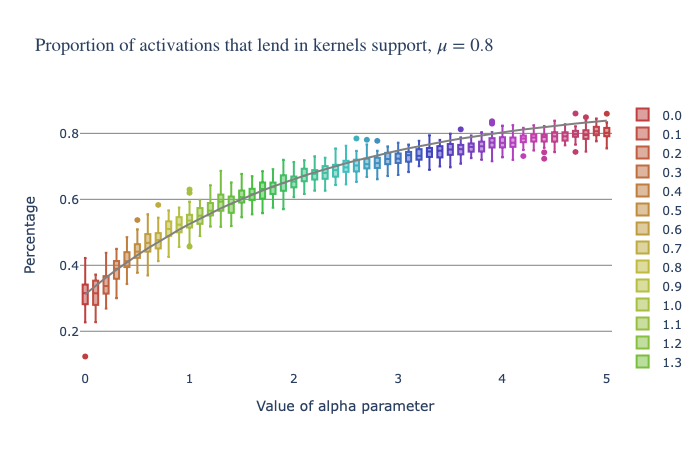
\includegraphics[scale=0.6]{pics/ppt_in_support_transp.png}
    \caption{Proportion of generated activations within $\mathcal{S}$ based on the $\alpha$ parameter, where $\mu=0.8, T=180, n_p=73, \intervalleFF{a}{b}=\bracks{30, 800} \num{e-3}$, with 50 simulations for each value of $\alpha$. In black, the function $f^{-1}(p_a)$.}
    \label{fig:ppt_in_support}
\end{figure}

As mentioned before, we are looking for a function, which, from the data, would allow us to have a first estimate of $\alpha$, in order to initialise the EM algorithm intuitively.
A first observation that can be made with the help of this figure is that there is most probably a relationship between the value of the coefficient $\alpha$ and $p_a$.
If we manage to establish such a relation, then, by taking its inverse, we will be able to determine a first value of $\alpha$ from the proportion $p_a$, which can be calculated immediately from the data.
We can then initiate $\alpha$ in the following way:
\begin{equation}
    \alpha^{(0)} = f(p_a)
\end{equation}

A first observation that can be made from the outset is that, whatever the values of the parameters, $\alpha$, $\mu$, $T$, etc., $p_a$ will always be below 1, by definition.
So, looking at the shape of the relationship in Figure~\ref{fig:ppt_in_support}, a first idea is the following:
\begin{equation}\label{eq:alpha_init_1}
    f(p_a) = -\ln \pars{1-p_a}
\end{equation}

When $\alpha = 0$, the intensity is reduced to its baseline, i.e., $\lambda_{k,p}(t) = \mu_k, \forall t \in \intervalleFF{0}{T}$, the proportion of acceptance in the simulation algorithm is therefore 1.
Thus, we find ourselves in the simple case of a simulation of a homogeneous Poisson process, i.e., with constant intensity.
Thus, the proportion of activations found in the supports of the different kernels must be simply equal to the proportion represented by all the supports in the total duration.
We note this proportion $p_s$:
\begin{equation}
    p_s \coloneqq \frac{n_p \pars{b-a}}{T}
\end{equation}

Replacing with the numerical values used for the Figure~\ref{fig:ppt_in_support} gives $p_s = 0.31$, which is consistent with the median obtained for $\alpha = 0$.

Thus, a second observation that can be made is that if $\alpha$ is always positive, then $p_a$ is always higher than $p_s$.
We then modify \ref{eq:alpha_init_1} accordingly:
\begin{equation}
    f(p_a) = -\ln\pars{1-p_a} + \ln\pars{1-p_s} = -\ln\pars{\frac{1 - p_a}{1 - p_s}}
\end{equation}

In addition, the stronger the baseline, the less $p_a$ increases, so we want the curvature to decrease when $\mu$ increases:
\begin{equation}
    f(p_a) = - e^{\mu} \ln\pars{\frac{1 - p_a}{1 - p_s}}
\end{equation}

Likewise, the higher $\mu$ is, the harder it is for $p_a$ to reach the limit of 1.
However, we do not consider values of $\alpha$ too high, in order to remain realistic, and so we especially want a good estimate of $\alpha$ for values lower than 5.
Therefore, we propose to adapt the limit according to $\mu$:
\begin{equation}
    f(p_a) = - e^{\mu} \ln\pars{\frac{l(\mu) - p_a}{l(\mu)  - p_s}}
\end{equation}
where $l(\mu)$ is a function which is worth 1 when $\mu = 0$ (in this case all the activations are in $\mathcal{S}$, $p_a = 1$), and which tends towards $p_s$ when $\mu$ increases (because we recall that $p_a$ cannot be systematically lower than $p_s$ for positive values of $\alpha$).

Thus, we propose:
\begin{equation}
    l(\mu) = \pars{\frac{e^{\mu}-1}{5} + \frac{1}{1-p_s}}^{-1} + p_s
\end{equation}

In order to test our initialisation function, and to show that it is better than chance, we calculate $\alpha^{(0)} = f(p_a)$, for different values of $\mu$ and $\alpha$, for 50 simulations each time.
The RMSE (\textit{Root Mean Square Error}) is then calculated.
The result is shown in Figure~\ref{fig:heatmap_alpha_init_rmse}.

\begin{figure}[h!]
    \centering
    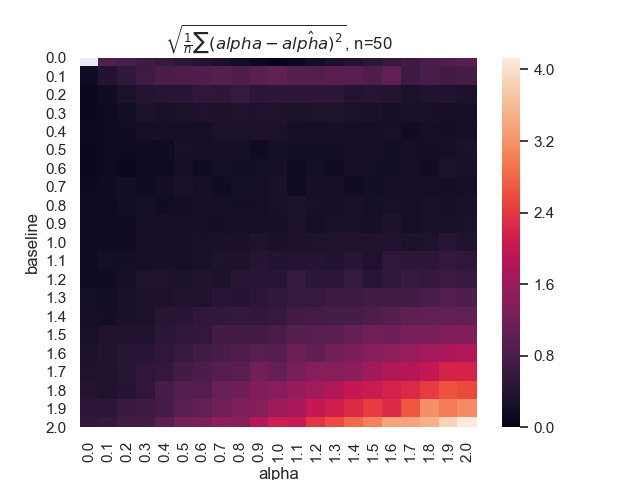
\includegraphics[scale=0.7]{pics/heatmap_baseline_alpha_alpha_init_rmse.jpg}
    \caption{RMSE between the calculated value for $\alpha^{(0)}$ and its true value, for different values of $\mu$ and $\alpha$.}
    \label{fig:heatmap_alpha_init_rmse}
\end{figure}

It can be seen from this figure that the estimate made of $\alpha$ is more than correct (i.e., cases where the RMSE is smaller than 1) in two main situations\footnote{We do not take into account the degenerate case where $\mu = \alpha = $0.}:
\begin{itemize}
    \item when the $\mu$ baseline is low, but greater than 0.2, for all values of $\alpha$; 
    \item when the $\alpha$ coefficient is low for all values in the baseline.
\end{itemize}

Conversely, the more $\mu$ and $\alpha$ increase simultaneously, the less accurate the initial estimate of $\alpha$ is.

There is a second degenerate case, in addition to the case where $\mu = \alpha = 0$: when $\mu = 0$ and $\alpha > 0$.
In this case, since the baseline is null, all activations are present on the kernel supports, because in the Algorithm~\ref{algo:1d_inhomogenous_pp}, if $s_{m+1} \notin \mathcal{S}$, then the intensity is null and therefore the probability of accepting such a point is also null.
Thus, we have $p_a = 1$, and $l(\mu) = 1$, and then $f(p_a)$ is worth $+\infty$.
So, when one is in this situation, one decides to return 1:
\begin{equation}
    f(p_a ; \mu, p_s) = 
    \left\{
		\begin{array}{ll}
			f(p_a) & \mbox{si } \mu > 0 \text{ ou } p_a > 0 \\
			1 & \mbox{sinon}
		\end{array}
	\right.
\end{equation}

\paragraph{Remark} In practice, the $\mu$ parameter of the function $f(p_a; \mu, p_s)$ is not the true value of the baseline, but the calculated value for its initialisation, as defined in Eq.~\eqref{eq:baseline_init}.



\section{Details of EM-based algorithm computations}\label{annexe:details_em}

Recall that we denote with the upper script the iteration step, e.g., $\theta^{(n)}$ is the value of the parameter $\theta$ at step $n$ of the EM algorithm.
By extension, if $f$ is a function of $\theta_1, \dots, \theta_m$, then we define $f^{(n)}\pars{\theta_1, \dots, \theta_m} \coloneqq f\pars{\theta_1^{(n)}, \dots, \theta_m^{(n)}}$.

Recall also that we defined $P_{t,k}^{(n)}$ and $P_{t,p}^{(n)}$ as follow:
\begin{equation*}
    P_{t,k} = \frac{\mu_k}{\lambda_{k,p}(t)}
\end{equation*}
\begin{equation*}
    P_{t,p} = \frac{\alpha_{k,p}\kappa_{k,p}\pars{t - t_*^{(p)}(t)}}{\lambda_{k,p}(t)}\1[t \geq t_1^{(p)}]
\end{equation*}

\paragraph{For $\mu_k$}
\begin{equation}
\begin{split}
    & \partiald{}{\mu_k}\mathcal{L}_{k,p}\pars{\mu_k, \alpha_{k,p}, m_{k,p}, \sigma_{k,p}} = 0 \\
    \Leftrightarrow &\sum_{t\in\mathcal{A}_k}\frac{1}{\lambda_{k,p}(t)} = T \\
    \Leftrightarrow &\sum_{t\in\mathcal{A}_k}\frac{P_{t,k}^{(n)}}{\mu_k} = T \\
    \Leftrightarrow &\mu_k^{(n+1)} = \frac{1}{T} \sum_{t\in\mathcal{A}_k} P_{t,k}^{(n)}
\end{split}
\end{equation}

\paragraph{For $\alpha_{k,p}$}
\begin{equation}
\begin{split}
    & \partiald{}{\alpha_{k,p}}\mathcal{L}_{k,p}\pars{\mu_k, \alpha_{k,p}, m_{k,p}, \sigma_{k,p}} = 0 \\
    \Leftrightarrow &\sum_{t\in\mathcal{A}_{k,p}}\frac{\kappa_{k,p}(t - t_*^{(p)}(t))}{\lambda_{k,p}(t)} = n_p \\
    \Leftrightarrow &\sum_{t\in\mathcal{A}_{k,p}}\frac{P_{t,p}^{(n)}}{\alpha_{k,p}} = n_p \\
    \Leftrightarrow &\alpha_{k,p}^{(n+1)} = \frac{1}{n_p} \sum_{t\in\mathcal{A}_{k,p}} P_{t,p}^{(n)}
\end{split}
\end{equation}

\paragraph{For $m_{k,p}$}
\begin{equation}
\begin{split}
    \partiald{}{m_{k,p}}\mathcal{L}_{k,p}\pars{\mu_k, \alpha_{k,p}, m_{k,p}, \sigma_{k,p}} &= -\sum_{t\in\mathcal{A}_{k,p}} \pars{\frac{t - t_*^{(p)}(t) - m_{k,p}}{\sigma_{k,p}^2} - \frac{C_m\pars{m_{k,p}, \sigma_{k,p},a,b}}{C\pars{m_{k,p}, \sigma_{k,p},a,b}}}\underbrace{\frac{\alpha_{k,p}\kappa_{k,p}(t)}{\lambda_{k,p}(t)}}_{=P_{t,p}} \\
    &= -\frac{1}{\sigma_{k,p}^2} \sum_{t\in\mathcal{A}_{k,p}} \pars{t - t_*^{(p)}(t)} P_{t,p} \\
    &+ \pars{\frac{m_{k,p}}{\sigma_{k,p}^2} + \frac{C_m\pars{m_{k,p}, \sigma_{k,p},a,b}}{C\pars{m_{k,p}, \sigma_{k,p},a,b}}} \sum_{t\in\mathcal{A}_{k,p}} P_{t,p}
\end{split}
\end{equation}
hence,
\begin{equation}
\begin{split}
    &\partiald{}{m_{k,p}}\mathcal{L}_{k,p}\pars{\mu_k, \alpha_{k,p}, m_{k,p}, \sigma_{k,p}} = 0 \\
    \Leftrightarrow &m_{k,p}^{(n+1)} = \frac{\sum_{t\in\mathcal{A}_{k,p}} \pars{t - t_*^{(p)}(t)} P_{t,p}^{(n)}}{\sum_{t\in\mathcal{A}_{k,p}} P_{t,p}^{(n)}} - {\sigma_{k,p}^{(n)}}^2 \frac{C_m\pars{m_{k,p}^{(n)}, \sigma_{k,p}^{(n)},a,b}}{C\pars{m_{k,p}^{(n)}, \sigma_{k,p}^{(n)},a,b}}
\end{split}
\end{equation}

\paragraph{For $\sigma_{k,p}$}
\begin{equation}
\begin{split}
    \partiald{}{\sigma_{k,p}}\mathcal{L}_{k,p}\pars{\mu_k, \alpha_{k,p}, m_{k,p}, \sigma_{k,p}} &= -\sum_{t\in\mathcal{A}_{k,p}} \pars{\frac{\pars{t - t_*^{(p)}(t) - m_{k,p}}^2}{\sigma_{k,p}^3} - \frac{C_\sigma\pars{m_{k,p}, \sigma_{k,p},a,b}}{C\pars{m_{k,p}, \sigma_{k,p},a,b}}}\underbrace{\frac{\alpha_{k,p}\kappa_{k,p}(t)}{\lambda_{k,p}(t)}}_{=P_{t,p}} \\
    &= -\frac{1}{\sigma_{k,p}^3} \sum_{t\in\mathcal{A}_{k,p}} \pars{t - t_*^{(p)}(t) - m_{k,p}}^2 P_{t,p} \\
    &+  \frac{C_\sigma\pars{m_{k,p}, \sigma_{k,p},a,b}}{C\pars{m_{k,p}, \sigma_{k,p},a,b}} \sum_{t\in\mathcal{A}_{k,p}} P_{t,p}
\end{split}
\end{equation}
hence,
\begin{equation}
\begin{split}
    &\partiald{}{\sigma_{k,p}}\mathcal{L}_{k,p}\pars{\mu_k, \alpha_{k,p}, m_{k,p}, \sigma_{k,p}} = 0 \\
    \Leftrightarrow &\sigma_{k,p}^{(n+1)} = \pars{\frac{C\pars{m_{k,p}^{(n)}, \sigma_{k,p}^{(n)},a,b}}{C_\sigma\pars{m_{k,p}^{(n)}, \sigma_{k,p}^{(n)},a,b}} \frac{\sum_{t\in\mathcal{A}_{k,p}} \pars{t - t_*^{(p)}(t) - m_{k,p}}^2 P_{t,p}^{(n)}}{\sum_{t\in\mathcal{A}_{k,p}}  P_{t,p}^{(n)}}}^{1/3}
\end{split}
\end{equation}

\paragraph{Link to gradient descent}
TODO: dire que l'on peut, pour les trois premiers coefficients, voir l'algorithme EM comme un GD (remttre rapidement la formule de mise à jour des coefs), où le step parameter $\nu$ vaut une certaine valeur

\begin{equation}
    \mu_k^{(n+1)} - \mu_k^{(n)} = -\frac{\mu_k^{(n)}}{T} \partiald{}{\mu_k}\mathcal{L}_{k,p}\pars{\mu_k, \alpha_{k,p}, m_{k,p}, \sigma_{k,p}}
\end{equation}

\begin{equation}
    \alpha_{k,p}^{(n+1)} - \alpha_{k,p}^{(n)} = -\frac{\alpha_{k,p}^{(n)}}{n_p} \partiald{}{\alpha_{k,p}}\mathcal{L}_{k,p}\pars{\mu_k, \alpha_{k,p}, m_{k,p}, \sigma_{k,p}}
\end{equation}

\begin{equation}
    \begin{split}
        m_{k,p}^{(n+1)} - m_{k,p}^{(n)} &=\frac{\sum_{t\in\mathcal{A}_{k,p}} \pars{t - t_*^{(p)}(t)} P_{t,p}^{(n)}}{\sum_{t\in\mathcal{A}_{k,p}} P_{t,p}^{(n)}} - {\sigma_{k,p}^{(n)}}^2 \frac{C_m\pars{m_{k,p}^{(n)}, \sigma_{k,p}^{(n)},a,b}}{C\pars{m_{k,p}^{(n)}, \sigma_{k,p}^{(n)},a,b}} - m_{k,p}^{(n)} \\
        &= \frac{1}{\sum_{t\in\mathcal{A}_{k,p}} P_{t,p}^{(n)}}\sum_{t\in\mathcal{A}_{k,p}} \pars{t - t_*^{(p)}(t) - {\sigma_{k,p}^{(n)}}^2 \frac{C_m\pars{m_{k,p}^{(n)}, \sigma_{k,p}^{(n)},a,b}}{C\pars{m_{k,p}^{(n)}, \sigma_{k,p}^{(n)},a,b}} - m_{k,p}^{(n)}} P_{t,p}^{(n)} \\
        &= \frac{{\sigma_{k,p}^{(n)}}^2}{\sum_{t\in\mathcal{A}_{k,p}} P_{t,p}^{(n)}} \sum_{t\in\mathcal{A}_{k,p}} P_{t,p}^{(n)} \pars{\frac{t - t_*^{(p)}(t) - m_{k,p}^{(n)}}{{\sigma_{k,p}^{(n)}}^2} - \frac{C_m\pars{m_{k,p}^{(n)}, \sigma_{k,p}^{(n)},a,b}}{C\pars{m_{k,p}^{(n)}, \sigma_{k,p}^{(n)},a,b}}} \\
        &= - \frac{{\sigma_{k,p}^{(n)}}^2}{\sum_{t\in\mathcal{A}_{k,p}} P_{t,p}^{(n)}} \partiald{}{m_{k,p}}\mathcal{L}_{k,p}\pars{\mu_k, \alpha_{k,p}, m_{k,p}, \sigma_{k,p}}
    \end{split}
\end{equation}



% Présentation nouvelles commandes
%\section*{Présentation et test des nouvelles commandes}

Cette section a pour but de montrer quelles sont les nouvelles commandes qui ont été ajoutées à ce document.

\subsection*{Commandes pour les mathématiques}
Commandes pour l'écriture des mathématiques, dans le fichier commandes\_math.tex

\paragraph{Les ensembles} 
\begin{itemize}
    \item \verb=\N=  : \N
    \item \verb=\Z= : \Z
    \item \verb=\Q= : \Q
    \item \verb=\R= : \R
    \item \verb=\Complex= : \Complex
\end{itemize}


\paragraph{Les encadrements} Ces commandes permettent d'avoir une unique commande pour un même type de séparateur, dont la taille s'ajuste automatiquement au contenu : 
\begin{itemize}
    \item \verb=\angles{x}= : $\angles{x}$ et $$\angles{\sum_{i = 0}^{n}}$$
    \item \verb=\braces{x}= : $\braces{x}$ et $$\braces{\sum_{i = 0}^{n}}$$
    \item \verb=\bracks{x}= : $\bracks{x}$ et $$\bracks{\sum_{i = 0}^{n}}$$
    \item \verb=\pars{x}= : $\pars{x}$ et $$\pars{\sum_{i = 0}^{n}}$$
    \item \verb=\norme{x}= : $\norme{x}$ et $$\norme{\sum_{i = 0}^{n}}$$
    \item \verb=\ent{x}= : $\ent{x}$ et $$\ent{\sum_{i = 0}^{n}}$$
    \item \verb=\entsup{x}= : $\entsup{x}$ et $$\entsup{\sum_{i = 0}^{n}}$$
    \item \verb=\abs{x}= : $\abs{x}$ et $$\abs{\sum_{i = 0}^{n}}$$
\end{itemize}

\paragraph{Les dérivées} Permet de gérer facilement les degrés de dérivation, ce dernier étant un argument optionnel, passé par défaut à vide :
\begin{itemize}
    \item \verb=\deriv{f(x)}{x}= : $$\deriv{f(x)}{x}$$
    \item \verb=\deriv[2]{f(x)}{x}= : $$\deriv[2]{f(x)}{x}$$
    \item \verb=\partiald{f(x)}{x}= : $$\partiald{f(x)}{x}$$
    \item \verb=\partiald[2]{f(x)}{x}= : $$\partiald[2]{f(x)}{x}$$
\end{itemize}

\paragraph{Intervalles} Différents types d'intervalles :
\begin{itemize}
    \item \verb=\intervalleOO{a}{b}= : $\intervalleOO{a}{b}$
    \item \verb=\intervalleFF{a}{b}= : $\intervalleFF{a}{b}$
    \item \verb=\intervalleOF{a}{b}= : $\intervalleOF{a}{b}$
    \item \verb=\intervalleFO{a}{b}= : $\intervalleFO{a}{b}$
    \item \verb=\intervalleEntier{a}{b}= : $\intervalleEntier{a}{b}$
\end{itemize}

\paragraph{Probabilités} Les notations utiles en probabilité (les arguments entre crochets sont optionnels, et peuvent donc être enlevés) : ce qui est valable pour \verb=\proba= l'est également pour \verb=\esp=, \verb=\var=, \verb=\cov= et \verb=\corr=.
\begin{itemize}
    \item \verb=\proba{}= : $\proba{}$
    \item \verb=\proba{X}= : $\proba{X}$
    \item \verb=\proba{X}[Y]= : $\proba{X}[Y]$
    \item \verb=\proba[\lambda]{X}[Y]= : $\proba[\lambda]{X}[Y]$
    \item \verb=\esp[\lambda]{X}[Y]= : $\esp[\lambda]{X}[Y]$
    \item \verb=\var[\lambda]{X}[Y]= : $\var[\lambda]{X}[Y]$
    \item \verb=\cov[\lambda]{X}{Y}[Z]= : $\cov[\lambda]{X}{Y}[Z]$
    \item \verb=\corr[\lambda]{X}{Y}= : $\corr[\lambda]{X}{Y}$
\end{itemize}

\paragraph{Lois de probabilités} Les différentes lois usuelles
\begin{itemize}
    \item \verb=\Ber{p}= : $\Ber{p}$
    \item \verb=\Binom{n}{p}= : $\Binom{n}{p}$
    \item \verb=\Poisson{\lambda}= : $\Poisson{\lambda}$
    \item \verb=\Geo{\lambda}= : $\Geo{\lambda}$
    \item \verb=\Unif{\intervalleFF{0}{1}}= : $\Unif{\intervalleFF{0}{1}}$
    \item \verb=\Exp{\lambda}= : $\Exp{\lambda}$
    \item \verb=\Norm[d]{\mu}{\sigma}= : $\Norm[d]{\mu}{\sigma}$
    \item \verb=\Gam{\alpha}{\theta}= : $\Gam{\alpha}{\theta}$
    \item \verb=\Betaloi{\alpha}{\theta}= : $\Betaloi{\alpha}{\theta}$
    \item \verb=\Pareto{r}{c}= : $\Pareto{r}{c}$
    \item \verb=\Laplace{\theta}= : $\Laplace{\theta}$
    \item \verb=\Cauchy{\theta}= : $\Cauchy{\theta}$
\end{itemize}


\paragraph{Égalités}
\begin{itemize}
    \item \verb=X \egalloi Y= : $X \egalloi Y$
    \item \verb=X \egalprob Y= : $X \egalprob Y $
    \item \verb=X \egaltxt{ipp} Y= : $X \egaltxt{ipp} Y $
    \item \verb=X \simiid Y= : $X \simiid Y $
\end{itemize}

\paragraph{max, min, argmax et argmin avec subscript} 
\begin{itemize}
    \item \verb=\maxx{x<2}= : $\maxx{x<2}$
    \item \verb=\minn{x<2}= : $\minn{x<2}$
    \item \verb=\argmax= : $\argmax$
    \item \verb=\argmax[x<2]= : $\argmax[x<2]$
    \item \verb=\argmin= : $\argmin$
    \item \verb=\argmin[x<2]= : $\argmin[x<2]$
\end{itemize}

\paragraph{Limites} Ce ne sont pas des nouvelles commandes, c'est juste pour rappel
\begin{itemize}
    \item \verb=\lim\limits_{x\to+\infty}= : $\lim\limits_{x\to+\infty}$
    \item \verb=\limsup\limits_{x\to+\infty}{f\pars{\frac{1}{x}}}= : $\limsup\limits_{x\to+\infty}{f\pars{\frac{1}{x}}}$
    \item \verb=\varliminf, \varlimsup,\varinjlim= : $\varliminf, \varlimsup,\varinjlim$
\end{itemize}

\paragraph{Matrices} Commandes pour matrices simples et vecteurs
\begin{itemize}
    \item \verb=\mattroisdiag{a}{b}{c}= : $$\mattroisdiag{a}{b}{c}$$
    \item \verb=\vecteur{AB}= : $$\vecteur{AB}$$
    \item \verb=\coord{AB}{12\\21}= : $$\coord{AB}{12\\21}$$
    \item \verb=\coord{BC}{21\\12\\32}= : $$\coord{BC}{21\\12\\32}$$
\end{itemize}


\paragraph{Intégration} La borne supérieure de l'intégrale est optionnelle
\begin{itemize}
    \item \verb=\dint x= : $\dint x$
    \item \verb=\integ{0}[+\infty]{f(x)}{x}= : $$\integ{0}[+\infty]{f(x)}{x}$$
    \item \verb=\integ{\mathcal{X}}{f(x)}{x}= : $$\integ{\mathcal{X}}{f(x)}{x}$$
\end{itemize}


\paragraph{Fonctions} Permet de définir rapidement une fonction

\verb=\fonction{f}{E}{F}{x}{f(x)}= : $$\fonction{f}{E}{F}{x}{f(x)}$$

\verb=\twopartdef{x}{x \geq 0}{-x}{x < 0}= : $$ \twopartdef { x } {x \geq 0} {-x} {x < 0}$$

\subparagraph{Remarque} Fonctionne de la même façon avec \verb=\threepartdef= puis en mettant 6 arguments au lieu de 4.

\paragraph{Divers}
\begin{itemize}
    \item \verb=\e{x}= : $\e{x}$
    \item \verb=\enstq{x}{x<2}= : $\enstq{x}{x<2}$
    \item \verb=\1= : $\1$
    \item \verb=\1[x<2]= : $\1[x<2]$
    \item \verb=\moy{x}= : $\moy{x}$
    \item \verb=\moyy{x}= : $\moyy{x}$
    \item \verb=\surf{10}= : $\surf{10}$
    \item \verb=\surf{10}[cm]= : $\surf{10}[cm]$
    \item \verb=\vol{10}= : $\vol{10}$
    \item \verb=\vol{10}[cm]= : $\vol{10}[cm]$
\end{itemize}


\subsection*{Commandes pour la \guill{typographie}}

Commandes pour le respect des règles typographiques françaises, et quelques abréviations.

\paragraph{Chiffres romains et siècle}
\begin{itemize}
    \item \verb=\cRM{5}= : \cRM{5}
    \item \verb=\cRm{5}= : \cRm{5}
    \item \verb=\crm{5}= : \crm{5}
    \item \verb=\siecle{1}= : \siecle{1}
    \item \verb=\siecle{5}= : \siecle{5}
\end{itemize}

\paragraph{Abréviations} Abréviations utiles, qui respectent les règles typographiques
\begin{itemize}
    \item \verb=\ssi= : \ssi
    \item \verb=\cad= : \cad
    \item \verb=\cf= : \cf
    \item \verb=\apjc= : \apjc
    \item \verb=\avjc= : \avjc
    \item \verb=\Mme Dupont= : \Mme Dupont
    \item \verb=\Mlle Dupont= : \Mlle Dupont
    \item \verb=\numero 5= : \numero 5
    \item \verb=\Num 5= : \Num 5
    \item \verb=\nums 5 et 6= : \nums 5 et 6
    \item \verb=\Nums 5 et 6= : \Nums 5 et 6
\end{itemize}

\paragraph{Autres} Quelques autres commandes utiles
\begin{itemize}
    \item \verb=\guill{texte entre guillemets français}= : \guill{texte entre guillemets français}
    \item \verb=\auteur{Victor}{Hugo}= : \auteur{Victor}{Hugo}
\end{itemize}






% Bibliographie
\newpage
\phantomsection
\addcontentsline{toc}{section}{References}
\bibliographystyle{alpha} % apalike, plain, alpha
\bibliography{references}

% Notes de synthèse
\begin{minipage}{0.45\textwidth}
  \begin{flushleft} \Large
    \textsc{Allain} Cédric
  \end{flushleft}
\end{minipage}
\begin{minipage}{0.45\textwidth}
  \begin{flushright} \Large
    ENSAE 3\up{e} année\\
    \textit{Stage de fin d'études}\\
    \textit{Année scolaire 2019/2020}
  \end{flushright}
\end{minipage}
	
{\centering

\vspace{1.5cm}
\HRule \\[0.5cm]
{\huge\bfseries Modélisation des dépendances temporelles dans la détection des modèles récurrents en électrophysiologie (M/EEG) \\ -- \\ \textit{Note de synthèse} \par}
\bigskip
\HRule \\[0.5cm]
\vspace{0.5cm}
}

\setlength{\parskip}{5pt}

%\begin{otherlanguage*}{french}
\selectlanguage{french}
\phantomsection
\addcontentsline{toc}{section}{Note de synthèse}
\section*{Première section}
Lorem ipsum dolor sit amet, consectetur adipiscing elit. Sed non risus. Suspendisse lectus tortor, dignissim sit amet, adipiscing nec, ultricies sed, dolor. Cras elementum ultrices diam. Maecenas ligula massa, varius a, semper congue, euismod non, mi. Proin porttitor, orci nec nonummy molestie, enim est eleifend mi, non fermentum diam nisl sit amet erat. Duis semper. Duis arcu massa, scelerisque vitae, consequat in, pretium a, enim. Pellentesque congue. Ut in risus volutpat libero pharetra tempor. Cras vestibulum bibendum augue. Praesent egestas leo in pede. Praesent blandit odio eu enim. Pellentesque sed dui ut augue blandit sodales. Vestibulum ante ipsum primis in faucibus orci luctus et ultrices posuere cubilia Curae; Aliquam nibh. Mauris ac mauris sed pede pellentesque fermentum. Maecenas adipiscing ante non diam sodales hendrerit.

\begin{itemize}
    \item item 1;
    \item item 2?
\end{itemize}

%\end{otherlanguage*}
\begin{minipage}{0.45\textwidth}
  \begin{flushleft} \Large
    \textsc{Allain} Cédric
  \end{flushleft}
\end{minipage}
\begin{minipage}{0.45\textwidth}
  \begin{flushright} \Large
    ENSAE 3\textsuperscript{rd} year\\
    \textit{Graduation internship}\\
    \textit{Academic year 2019/2020}
  \end{flushright}
\end{minipage}
	
{\centering

\vspace{1.5cm}
\HRule \\[0.5cm]
{\huge\bfseries Modeling Temporal Dependencies between Recurring Patterns in Electrophysiology (M/EEG) \\ -- \\ \textit{Summary note} \par}
\bigskip
\HRule \\[0.5cm]
\vspace{0.5cm}
}

\setlength{\parskip}{5pt}

\selectlanguage{english}
\phantomsection
\addcontentsline{toc}{section}{Summary note}
\section*{First section}
Lorem ipsum dolor sit amet, consectetur adipiscing elit. Sed non risus. Suspendisse lectus tortor, dignissim sit amet, adipiscing nec, ultricies sed, dolor. Cras elementum ultrices diam. Maecenas ligula massa, varius a, semper congue, euismod non, mi. Proin porttitor, orci nec nonummy molestie, enim est eleifend mi, non fermentum diam nisl sit amet erat. Duis semper. Duis arcu massa, scelerisque vitae, consequat in, pretium a, enim. Pellentesque congue. Ut in risus volutpat libero pharetra tempor. Cras vestibulum bibendum augue. Praesent egestas leo in pede. Praesent blandit odio eu enim. Pellentesque sed dui ut augue blandit sodales. Vestibulum ante ipsum primis in faucibus orci luctus et ultrices posuere cubilia Curae; Aliquam nibh. Mauris ac mauris sed pede pellentesque fermentum. Maecenas adipiscing ante non diam sodales hendrerit.

\begin{itemize}
    \item item 1;
    \item item 2?
\end{itemize}

\end{document}
